\documentclass[12pt, twoside]{report}
\usepackage[a4paper,left=2cm, right=2cm, top=3cm,bottom=2cm]{geometry}
\usepackage[utf8]{inputenc}

\usepackage[english]{babel}
\usepackage{amsmath}
\usepackage{graphicx}
\usepackage{textcomp}
\usepackage{parskip}
\usepackage[colorinlistoftodos]{todonotes}
\usepackage{csquotes}
\usepackage{float}
\usepackage[backend=biber,style=ieee]{biblatex}
\usepackage{hyperref}
\usepackage{graphicx}
\usepackage{epsfig}
\usepackage{caption}
\usepackage{ragged2e}
\usepackage{subcaption}
\usepackage[singlespacing]{setspace}
\usepackage{hyperref}
\usepackage[utf8]{inputenc}
\usepackage[backend=biber,style=ieee]{biblatex}
\usepackage[paper=portrait,pagesize]{typearea}
\usepackage{pdflscape}

\usepackage{biblatex}

\usepackage{diagbox} %table split headers
\usepackage{longtable} %multi-page tables

\newcommand{\tabred}{-4pt}
\newcommand*\rot{\rotatebox[x=1.32cm]{90}}

\usepackage{makecell}
\usepackage[table,xcdraw]{xcolor}
\usepackage{tabularx}
% If you use beamer only pass "xcolor=table" option, i.e. \documentclass[xcolor=table]{beamer}
%\usepackage[normalem]{ulem}
\useunder{\uline}{\ul}{}


%\addbibresource{friedt.bib}
\addbibresource{OCT_ref.bib}
\setlength {\marginparwidth }{2cm} 

%Chapter and name in the same line
\usepackage{titlesec}
\titleformat{\chapter}[hang] 
{\normalfont\huge\bfseries}{\chaptertitlename\ \thechapter:}{1em}{} 

\titleformat{\chapter}[display]
  {\normalfont\bfseries}{}{0pt}{\Huge}
  

\usepackage{listings}
\definecolor{mygreen}{rgb}{0,0.6,0}
\definecolor{mygray}{rgb}{0.5,0.5,0.5}
\definecolor{mymauve}{rgb}{0.58,0,0.82}
\lstset{ 
  language=Octave,
  backgroundcolor=\color{white},
  basicstyle=\footnotesize,       
  breakatwhitespace=false,         
  breaklines=true,
  captionpos=b,
  commentstyle=\color{mygreen},    
  deletekeywords={...},         
  escapeinside={\%*}{*)},        
  extendedchars=false,              
  frame=single,	                  
  keepspaces=true,                 
  keywordstyle=\color{blue},                       
  morekeywords={*,...},          
  numbers=left,                    
  numbersep=5pt,                   
  numberstyle=\tiny\color{mygray}, 
  rulecolor=\color{black},        
  showspaces=false,               
  showstringspaces=false,        
  showtabs=false,                
  stepnumber=1,                    
  stringstyle=\color{mymauve},     
  tabsize=2,	                   
  title=\lstname                   
}

\usepackage{stackengine}

\newcommand\barbelow[1]{\stackunder[1.2pt]{$#1$}{\rule{.8ex}{.075ex}}}




\begin{document}


\lstset{language=Octave}
\begin{titlepage}

\newcommand{\HRule}{\rule{\linewidth}{0.5mm}}
\center 

\textsc{\LARGE Université Bourgogne Franche-Comté}\\[1.5cm] 
\textsc{\Large Master 2 in Smart Integrated Systems}\\[0.5cm] 

\HRule \\[0.4cm]
{ \huge \bfseries Report of Micro-robotics}\\[0.4cm] 
\HRule \\[1.5cm]


\includegraphics[scale=0.3]{logo_ubfc.png}\\[1cm]

\begin{center}

\begin{tabular}{ c   |   c } 
   
    %Opcion 2:
    ARUQUIPA Grover & \normalsize \href{mailto:grover.grover_aruquipa_aruquipa@edu.univ-fcomte.fr}{grover.grover \textunderscore aruquipa \textunderscore aruquipa@edu.univ-fcomte.fr}\\
    MEZIANE Sameh &  \normalsize \href{mailto:sameh.meziane@edu.univ-fcomte.fr}{sameh\textunderscore  meziane@edu.univ-fcomte.fr}
    
\end{tabular}
\end{center}

\vfill
{\large \today}\\[1cm] 
\vfill 

\end{titlepage}
 

%\thispagestyle{empty}
%\tableofcontents
%\listoffigures
\pagebreak
\chapter{TP 1: \LARGE Concentric Tube Robot}
Link of the code implementation \footnote{Repository of the Tps \url{https://github.com/GroverAruquipa/Micro_robotics_TPs}.}\\
\section{Introduction}
A concentric tubes robot is a type of robot that has multiple tubes around a central axis. These tubes can be used for a variety of purposes, such as moving objects or providing a path for fluids.

Concentric tubes robots are becoming increasingly popular due to their versatility and ability to be adapted for a variety of tasks. They are often used in manufacturing and laboratory settings, where they can be used to move or handle objects. In addition, they can be used to transport fluids, which can be important in medical and laboratory settings.

There are a number of different types of concentric tubes robots, each with its own advantages and disadvantages. Some of the most common types include:
\begin{itemize}
    \item Pneumatic tubes: These robots use pressurized air to move objects or fluids through the tubes. This type of robot is relatively simple and inexpensive to build, but it can be difficult to control the movement of objects or fluids.
    \item Robotic arms: These robots use a number of tubes to create a robotic arm. This type of robot is more complex than pneumatic robots, but it can be used to more accurately control the movement of objects or fluids.
    \item Fluidic robots: These robots use a number of tubes to create a network of fluid channels. This type of robot is extremely complex, but it can be used to accurately control the movement of fluids.
\end{itemize}

\section{Exercise 1. Establishing the kinematic model : arc parameter model or $f_{independient}$}
\subsection{What are the transformations between the coordinate frame $j-1$ and $j$ in Figure 2a  ?}
The transformation is defined using the transformation matrices as is observed in\ref{eq:trans1}, where its possible to observe the rotations around $z$, $y$ and additionally the translations in $y$.

\begin{equation}
    ^{j-1} T_{j}=\begin{bmatrix}
        R_{z}(\phi_j) & 0 \\
        0 & 1
    \end{bmatrix} \begin{bmatrix}
        R_{y}(\theta_j) & p_j \\
        0 & 1
    \end{bmatrix} 
    \label{eq:trans1}
\end{equation}

Where $\theta_{j} = k_{j} l_{j}$ and $p_{j}=[r_{j}(1-cos(\theta_j)), 0, r_{j}sin(\theta_j)]^T$ and $r_{j}=[1/k_{j},0,0]^T$, so that the rotation around the y axis is defined by $\theta_j$ and the rotation around the z axis is defined as $\phi_{j}$
So that the transformation matrix will be defined as:\\


\subsection{Calculate the homogeneous transformation matrix of the coordinate frame of the section $j-1$ to section $j$}
The homogeneous transformation will be defines as Eq. \ref{eq:homogen}, where we can observe the final transformation matrix.\\


\begin{equation}
    T=\begin{bmatrix}
        cos(\phi)cos(ks) & -sin(\phi) &cos(\phi) sin(ks)& \dfrac{cos(\phi)(1-cos(ks))}{k}\\
        
        sin(\phi)cos(ks) & cos(\phi) & sin(\phi)sin(ks) &  \dfrac{sin(\phi)(1-cos(ks))}{k}\\
        -sin(ks) & 0 & cos(ks) & \dfrac{sin(ks)}{k}\\
        0 & 0 & 0 & 1
    \end{bmatrix}
    \label{eq:homogen}
\end{equation}
Additionally we can define the vector trajectory using the Eq. \ref{eq:homogen}, which will help us to find the  $x,y,z$ in the space.\\ 
\begin{equation}
    p=\begin{bmatrix}
        \dfrac{1}{k}(1-cos(\theta)\\
        0\\
        \dfrac{1}{k} sin(\theta)\\
        0
    \end{bmatrix}
    \label{eq:traj}
\end{equation}

And additionally for the extrusion we can define the rotation around the axis $z$ as is observed below in the Eq. \ref{eq:rotz}\\
\begin{equation}
    Rz_{\phi}=\begin{bmatrix}
        cos(\phi) &-sin(\phi) &0 &0 \\
        sin(\phi) & cos(\phi) & 0 & 0 \\
        0 & 0 & 1 & 0 \\
        0 & 0 & 0 &1 \\
    \end{bmatrix}
    \label{eq:rotz}
\end{equation}


\subsection{Determine the transformation matrix from the robot base to the effector $^0 T_e$ of two and three
section robots. It corresponds to $f_{independent}$ of CTR model}
In this section we present the transformation matrices for each tube as is shown below:\\
For $^0 T_1$, we can obtain:\\
\begin{equation}
    ^0 T_1=\begin{bmatrix}
        cos(\phi_1)cos(k_1 s_1 ) & \sin(\phi_1) &cos(\phi_1) sin(k_1 s_1)& \dfrac{cos(\phi_1)(1-cos(k_1 s_1))}{k_1}\\
        
        sin(\phi_1)cos(k_1 s_1) & cos(\phi_1) & sin(\phi_1)sin(k_1 s_1) &  \dfrac{sin(\phi_1)(1-cos(k_1 s_1))}{k_1}\\
        -sin(k_1 s_1) & 0 & cos(k_1 s_1) & \dfrac{sin(k_1 s_1)}{k_1}\\
        0 & 0 & 0 & 1
    \end{bmatrix}
    \label{eq:homogen1}
\end{equation}

For $^1 T_2$, we can obtain:\\
\begin{equation}
    ^1 T_2=\begin{bmatrix}
        cos(\phi_2)cos(k_2 s_2 ) & \sin(\phi_2) &cos(\phi_2) sin(k_2 s_2)& \dfrac{cos(\phi_2)(1-cos(k_2 s_2))}{k_2}\\
        
        sin(\phi_2)cos(k_2 s_2) & cos(\phi_2) & sin(\phi_2)sin(k_2 s_2) &  \dfrac{sin(\phi_2)(1-cos(k_2 s_2))}{k_2}\\
        -sin(k_2 s_2) & 0 & cos(k_2 s_2) & \dfrac{sin(k_2 s_2)}{k_2}\\
        0 & 0 & 0 & 1
    \end{bmatrix}
    \label{eq:homogen1}
\end{equation}

For $^2 T_3$, we can obtain:\\
\begin{equation}
    ^1 T_3=\begin{bmatrix}
        cos(\phi_3)cos(k_3 s_3 ) & \sin(\phi_3) &cos(\phi_3) sin(k_3 s_3)& \dfrac{cos(\phi_3)(1-cos(k_3 s_3))}{k_3}\\
        
        sin(\phi_3)cos(k_3 s_3) & cos(\phi_3) & sin(\phi_3)sin(k_3 s_3) &  \dfrac{sin(\phi_3)(1-cos(k_3 s_3))}{k_3}\\
        -sin(k_3 s_3) & 0 & cos(k_3 s_3) & \dfrac{sin(k_3 s_3)}{k_3}\\
        0 & 0 & 0 & 1
    \end{bmatrix}
    \label{eq:homogen1}
\end{equation}
In consequence the final transformation will be defined as:\\

\begin{equation}
    ^0 T_e=^{0} T_{1} * ^{1} T_{2} * ^{2} T_{3}
\end{equation}
Additionally its possible to observe how the model is presented as the previous section.

\subsection{With the function $extrude.m$, plot various shape of the robot in 4 different configurations $l_1 , \phi_1 , \theta_1 ,l_2 , \phi_2 , \theta_2 $}
In order to define this function, firstly we can define the parameters for the 3 tubes as:
\begin{lstlisting}
    dr=pi/200; %rotation angle 
    R1=2.8e-3; %radius of the external tube 1
    r1=2.5e-3; %radius of the internal tube 1
    k1=-100; %60%10 %curvature of the tube 
    phi_1=2*dr; %angle of the tube
    l1=0.02; %length of the tube
    R2=2.1e-3; %radius of the external tube 2
    r2=1.9e-3; %radius of the internal tube 2
    k2=30; %curvature of the tube
    phi_2=60*dr; %Angle rotation of the tube  
    l2=0.02; %Section length of the tube 2
\end{lstlisting}
Using the previous parameters in order to find the tube 1, we can define as follows: \\
\begin{lstlisting}
    %Axis 1
    T1=transform(phi_1, k1, l1); % this function is used to calculate the transformation matrix
    T=T1; %T is the transformation matrix
    r11=1/k1; %radius of the tube
    theta_1=k1*l1; %angle of the tube
    theta_range=linspace(0,theta_1,20); %range of the angle
    P1=translation_concentric(r11,theta_range); %P1=[r11*(1-cos(theta_range)); theta_range*0; r11*sin(theta_range); 1+theta_range*0];
    Rz=[cos(phi_1) -sin(phi_1) 0 0; sin(phi_1) cos(phi_1) 0 0; 0 0 1 0; 0 0 0 1]; %Rotation matrix
    traj=Rz*P1; %traj is the trajectory of the tube
    traj1=traj(1:3,:); %traj1 is the trajectory of the tube in the x,y,z plane
    c1=linspace(0, 2*pi, 20); %range of the angle
    int1=r1*[cos(c1); sin(c1)]; %int1 is the internal tube
    ext1=R1*[cos(c1); sin(c1)]; %ext1 is the external tube
    [X,Y,Z]=extrude(int1,traj1); %this function is used to create the tube
    figure(1)
    surf(X,Y,Z); %axis equal; hold on;
    [X1,Y1,Z1]=extrude(ext1,traj1);
    surf(X1,Y1,Z1); %axis equal; hold on;
    hold on
\end{lstlisting}
Additionally for the tube 2 its possible to define a similiar code with the previous parameters defined.\\
\begin{lstlisting}
    %% Axis 2  
    theta2=k2*l2;
    r22=1/k2;
    theta_range2=linspace(0,theta2,20);
    T2=transform(phi_2, k2, l2);
    P2=translation_concentric(r22,theta_range2); %P2=[r22*(1-cos(theta_range2)); theta_range2*0; r22*sin(theta_range2); 1+theta_range2*0];
    Rz2=[cos(phi_2) -sin(phi_2) 0 0; sin(phi_2) cos(phi_2) 0 0; 0 0 1 0; 0 0 0 1];
    traj2=T1*Rz2*P2;
    traj22=traj2(1:3,:);
    c2=linspace(0, 2*pi, 20);
    int2=r2*[cos(c2); sin(c2)];
    ext2=R2*[cos(c2); sin(c2)];
    [X2,Y2,Z2]=extrude(int2,traj22);
    surf(X,Y,Z);% axis equal; hold on;
    [X22,Y22,Z22]=extrude(ext2,traj22);
    surf(X22,Y22,Z22);% axis equal; hold on;
\end{lstlisting}


After applying, the due transformations and in the same way coding the model or equivalences of the curvature and elongation we can obtain the following results:\\
\begin{figure}[H]
     \centering
     \begin{subfigure}[b]{0.3\textwidth}
         \centering
         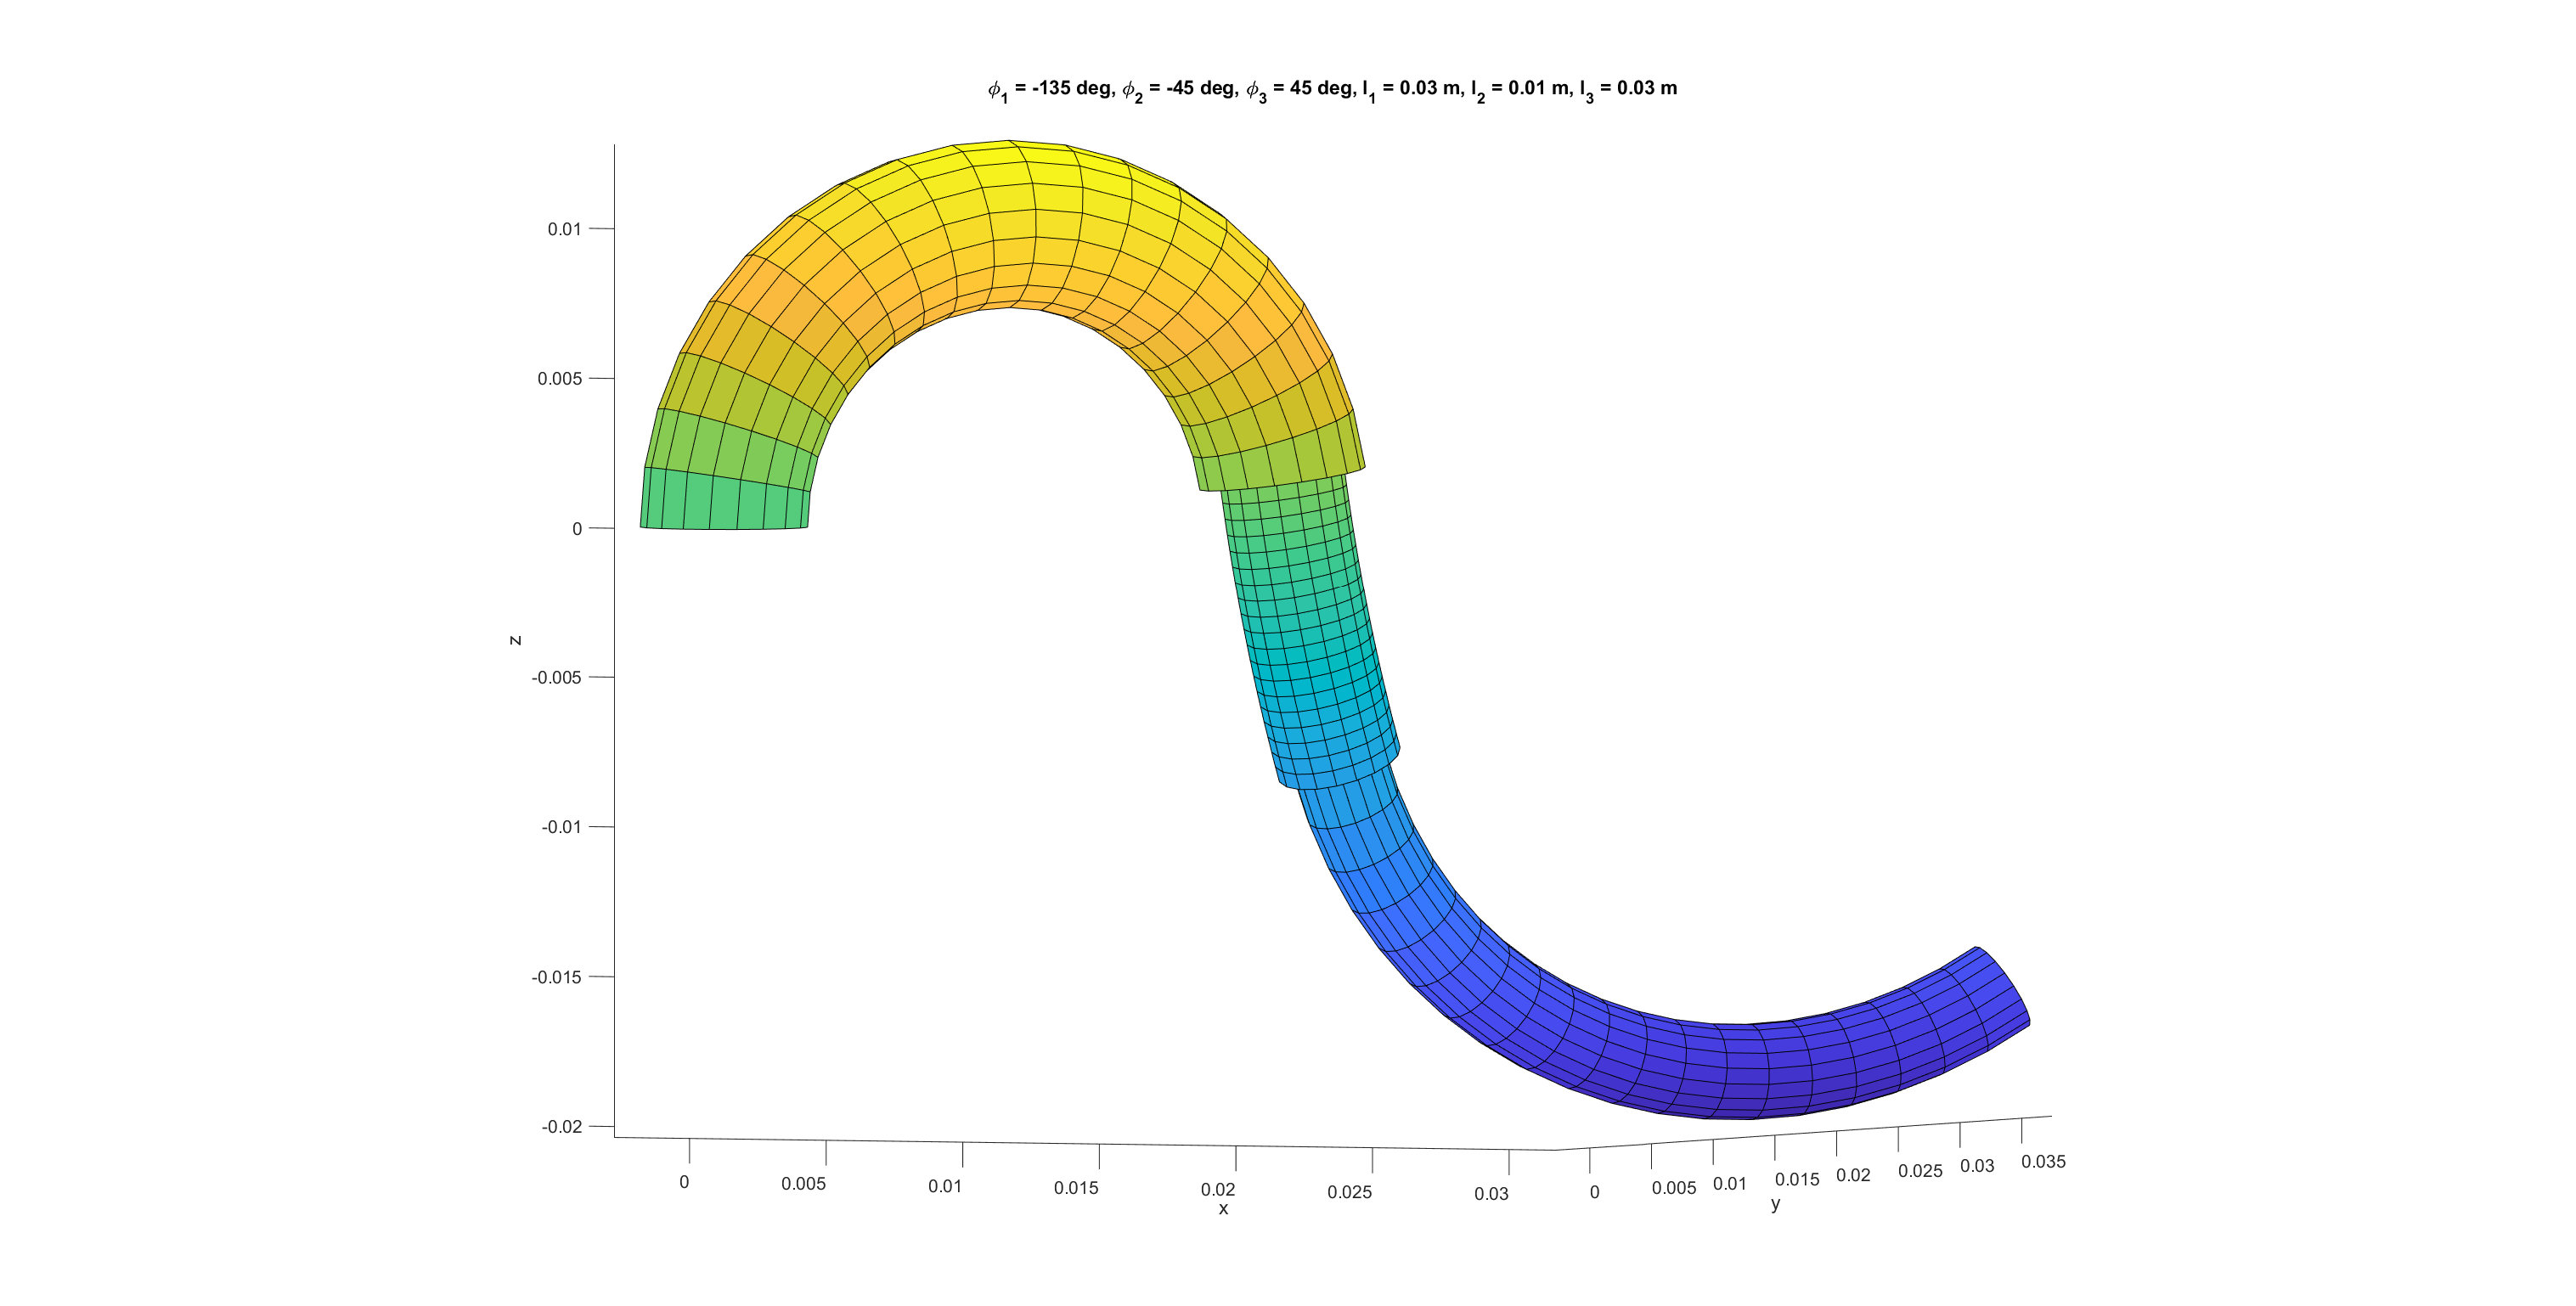
\includegraphics[width=\textwidth]{TP_1/sample6.eps}
         \caption{First Configuration}
         \label{figtube1}
     \end{subfigure}
     \hfill
     \begin{subfigure}[b]{0.3\textwidth}
         \centering
         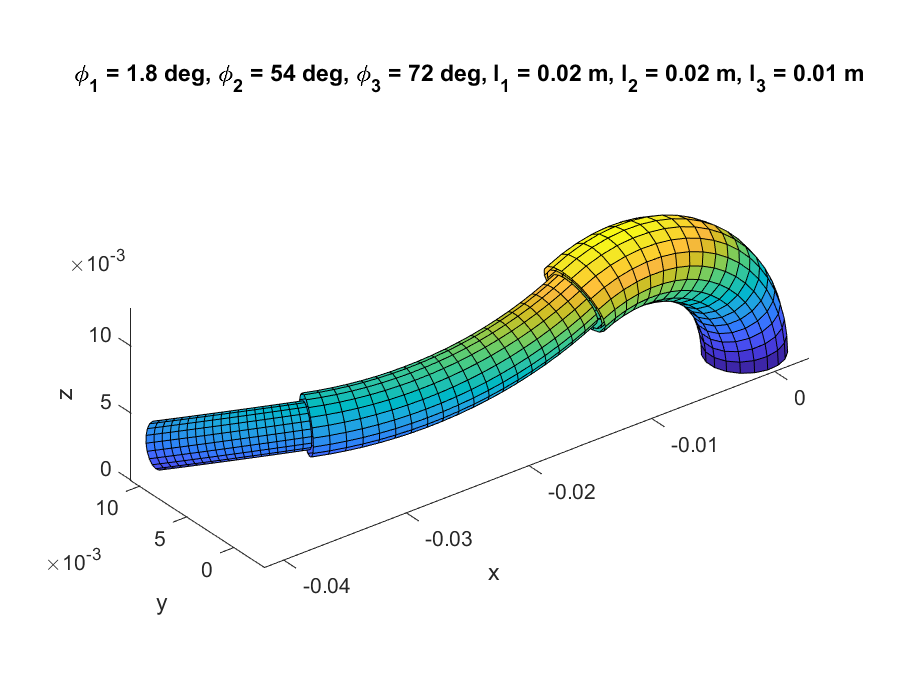
\includegraphics[width=\textwidth]{TP_1/sample1.eps}
         \caption{Second Configuration}
         \label{fig:tube2}
     \end{subfigure}
     \hfill
     \begin{subfigure}[b]{0.3\textwidth}
         \centering
         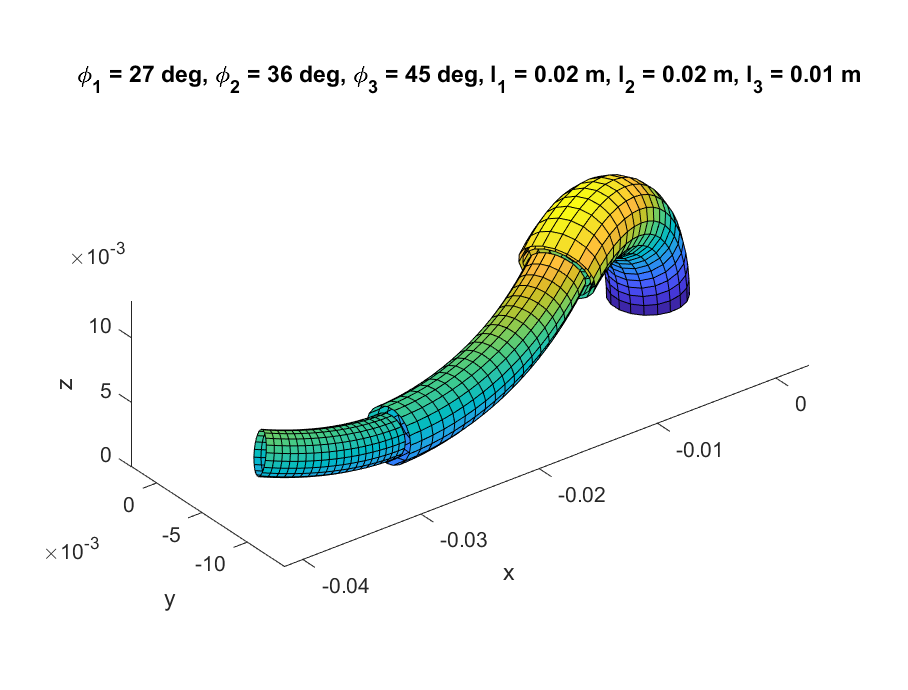
\includegraphics[width=\textwidth]{TP_1/sample2.eps}
         \caption{Third Configuration}
         \label{fig:Tube3}
     \end{subfigure}
      \hfill
     \begin{subfigure}[b]{0.3\textwidth}
         \centering
         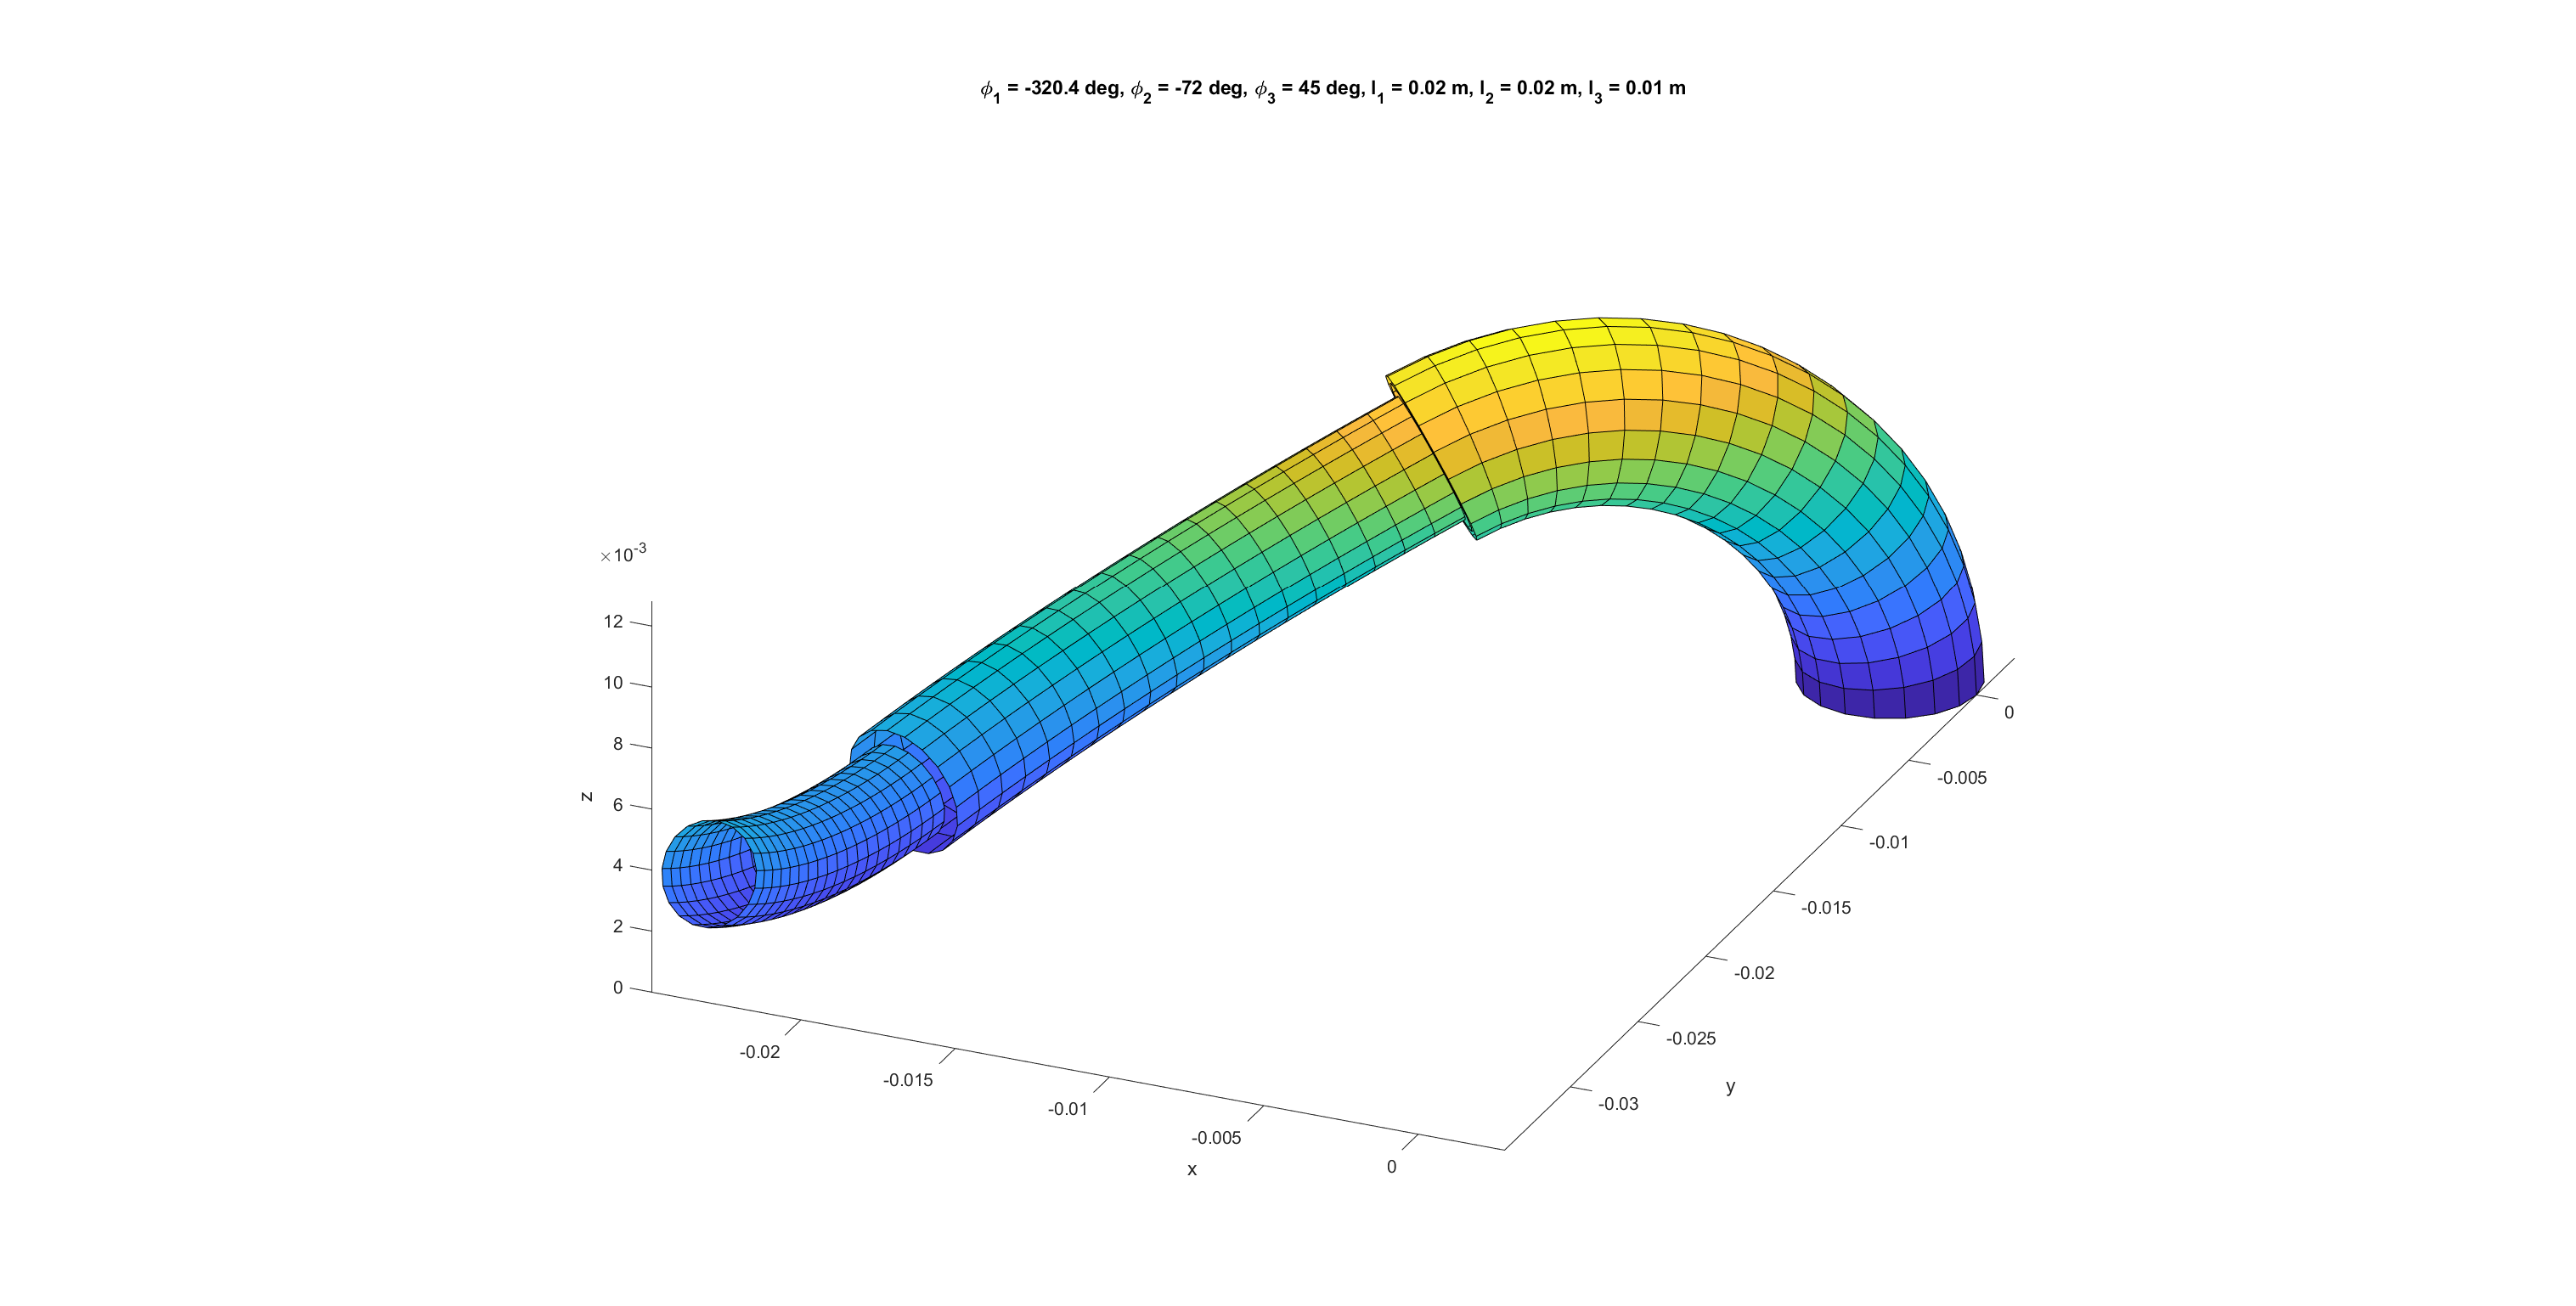
\includegraphics[width=\textwidth]{TP_1/sample3.eps}
         \caption{fourth Configuration}
         \label{fig:Tube4}
     \end{subfigure}
      \hfill
     \begin{subfigure}[b]{0.3\textwidth}
         \centering
         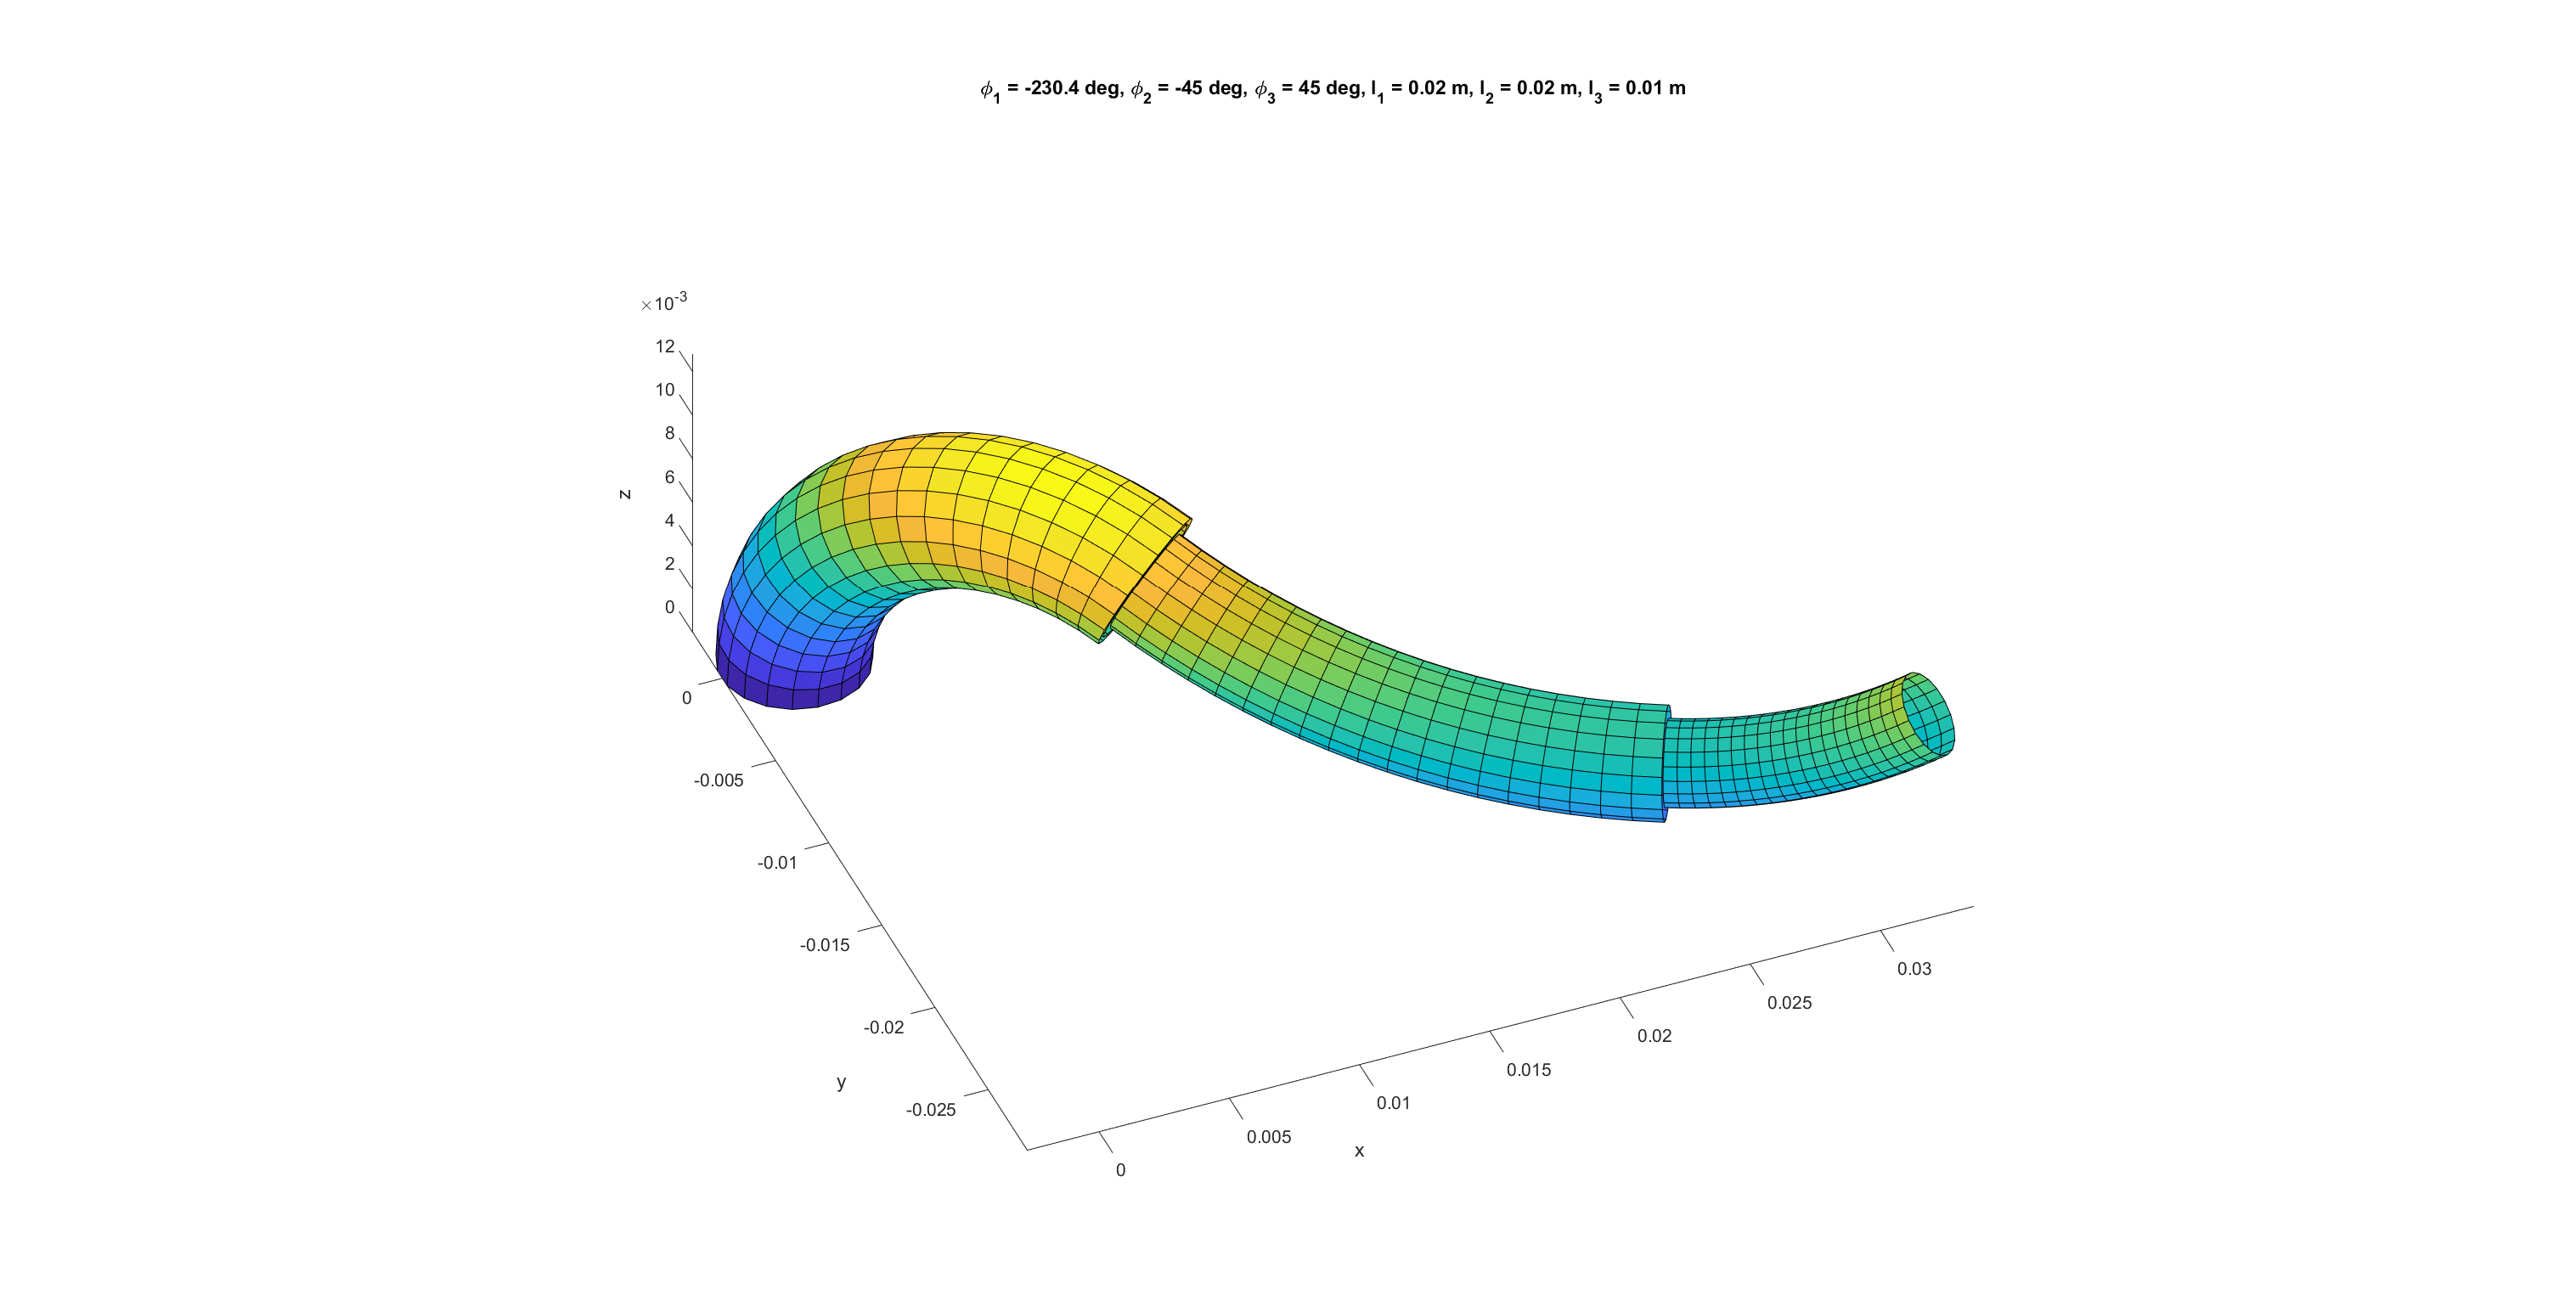
\includegraphics[width=\textwidth]{TP_1/sample4.eps}
         \caption{fifth Configuration}
         \label{fig:Tube5}
     \end{subfigure}
    \hfill
     \begin{subfigure}[b]{0.3\textwidth}
         \centering
         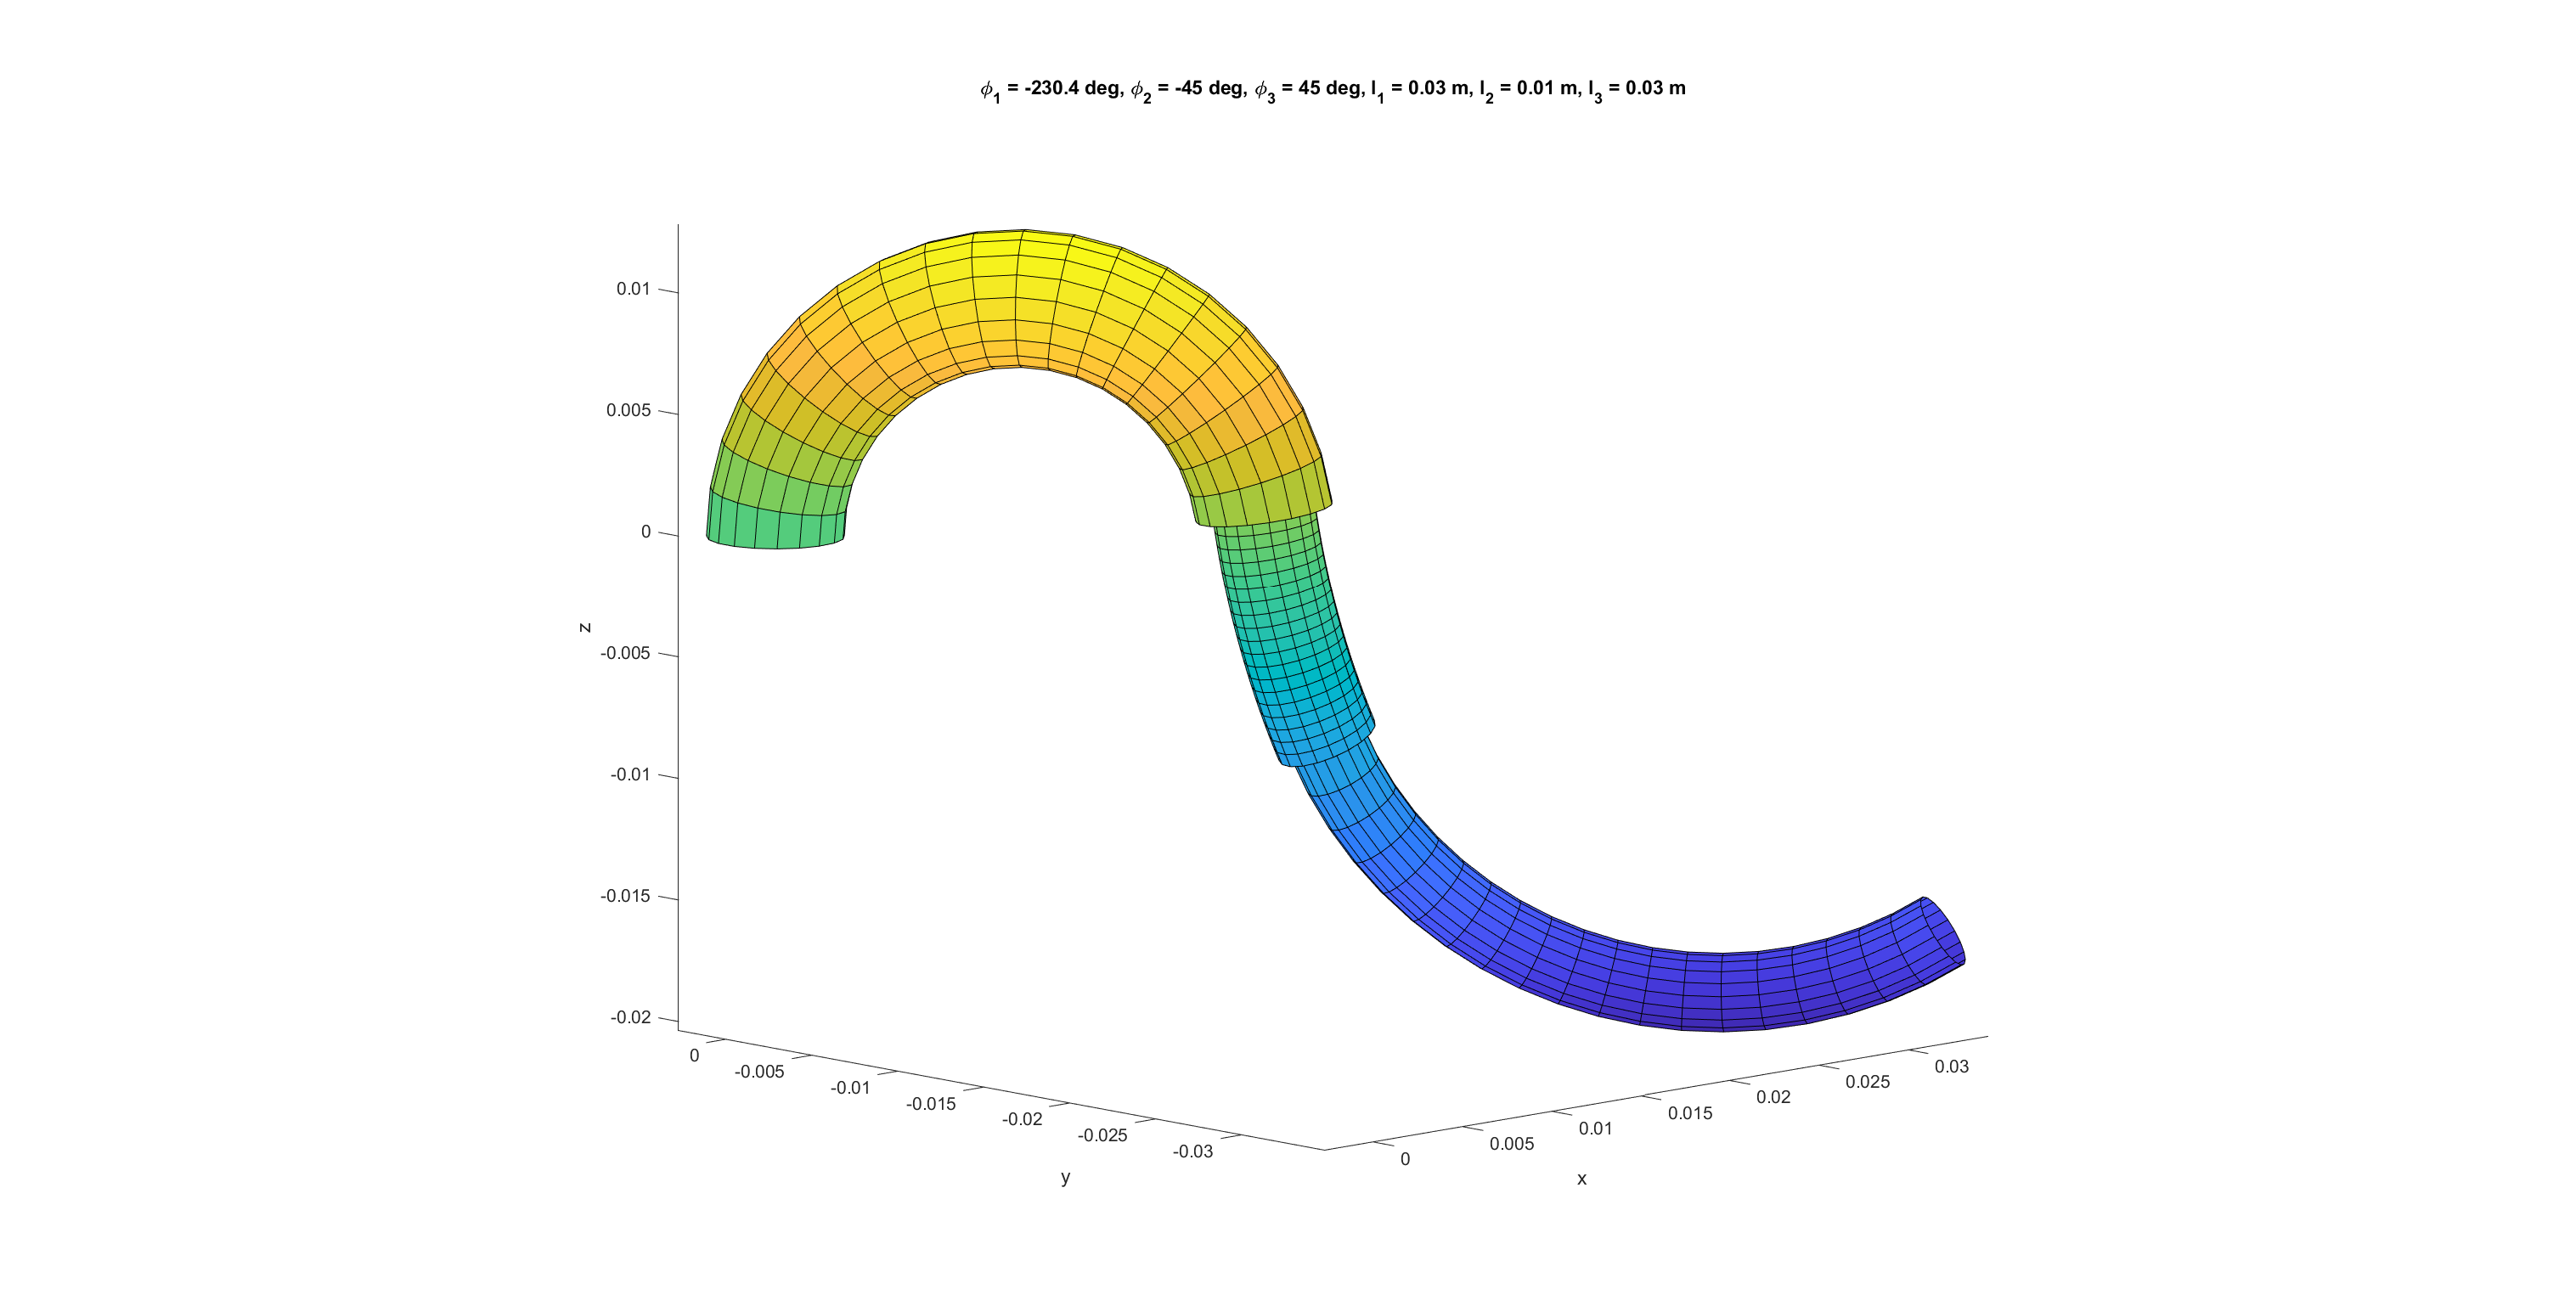
\includegraphics[width=\textwidth]{TP_1/sample5.eps}
         \caption{sixth Configuration}
         \label{fig:Tube6}
     \end{subfigure}
        \caption{6 tubes}
        \label{fig:tubes}
\end{figure}

In the Fig. \ref{fig:tubes}, we can observe the different configurations presented, modifying them randomly for different curvatures and elongations, it is possible to observe how the transformations for each tube are respected, which shows a correct implementation of this type of robot in the simulation software.





\section{Exercise 2.Establishing the section model : $f_{specific}$}
Find attached the codes of the curse in the Link \footnote{Repository of the Tps \url{https://github.com/GroverAruquipa/Micro_robotics_TPs}.}

\subsection{Implement these functions for your three tubes CTR prototypes}
\begin{lstlisting}
    
L=[64e-3 200.5e-3]; % Length of the tube
OD=[1.07e-3 0.65e-3]; % Outer diameter of the tube
ID=[0.77e-3 0.42e-3]; % Inner diameter of the tube
uix=[14.4 11.02]; % Planar curvature of the tube
k=[14.4 11.02]
kbi=[3.89e-4 2.00e-3]; % Relative permeability of the tube
deni=[6.45e3 6.45e3]; % Density of the tube
T=[0.02 0.3];
n=2;
% Ei is the elastic modulus of the tube
%calculate Ei 
Ei=deni.*(OD.^4-D.^4)/32;
E=80e9; % Elastic modulus of the steel tube Gpa 
Ei=[E E]; % Elastic modulus of the tube
I=D.^4/64; % Cross sectional inertia of the tube size 1x2
R=[pi/4 pi/4;]
Linit=[0.2 0.1]
% I is the cross sectional inertia of the tube
%calculate I
I=deni.*(OD.^4-D.^4)/64;
% To calculate kx and ky with n=2

[phi, curv, L]=f_specific(T,R, Linit,E ,ID, OD, k)
\end{lstlisting}

\begin{center}
    
\begin{table}[H]
\caption{Results of the calculation for each tube}
\centering
\begin{tabular}{|c|c|c|l|}
\hline
{\ul \textbf{}} & {\ul \textbf{t}} & {\ul \textbf{c}} & d \\ \hline
\textbf{Tube 1} &     $0.6123X10^{-6}$       &  13.9428               & 0.12  \\ \hline
\textbf{Tube 2} &   $0.6123X10^{-6}$               & 11.02                 &   0.125\\ \hline
\end{tabular}
\end{table}
\end{center}


\subsection{Measure φi(q), κi(q), and ‘i(q) for at least five configurations of the robot. Each configuration
has to be in plane in order to perform the measurement through camera. Use the circfit.m function to
derive and plot the radius of curvature $ki(q)$.}

% sameh
In this section we present a number of images taken from a tube concentric robot prototype, in order to calculate its curvature taking into account different points and seeking to obtain them through a regression.

\begin{figure}[H]
     \centering
     \begin{subfigure}[b]{0.3\textwidth}
         \centering
         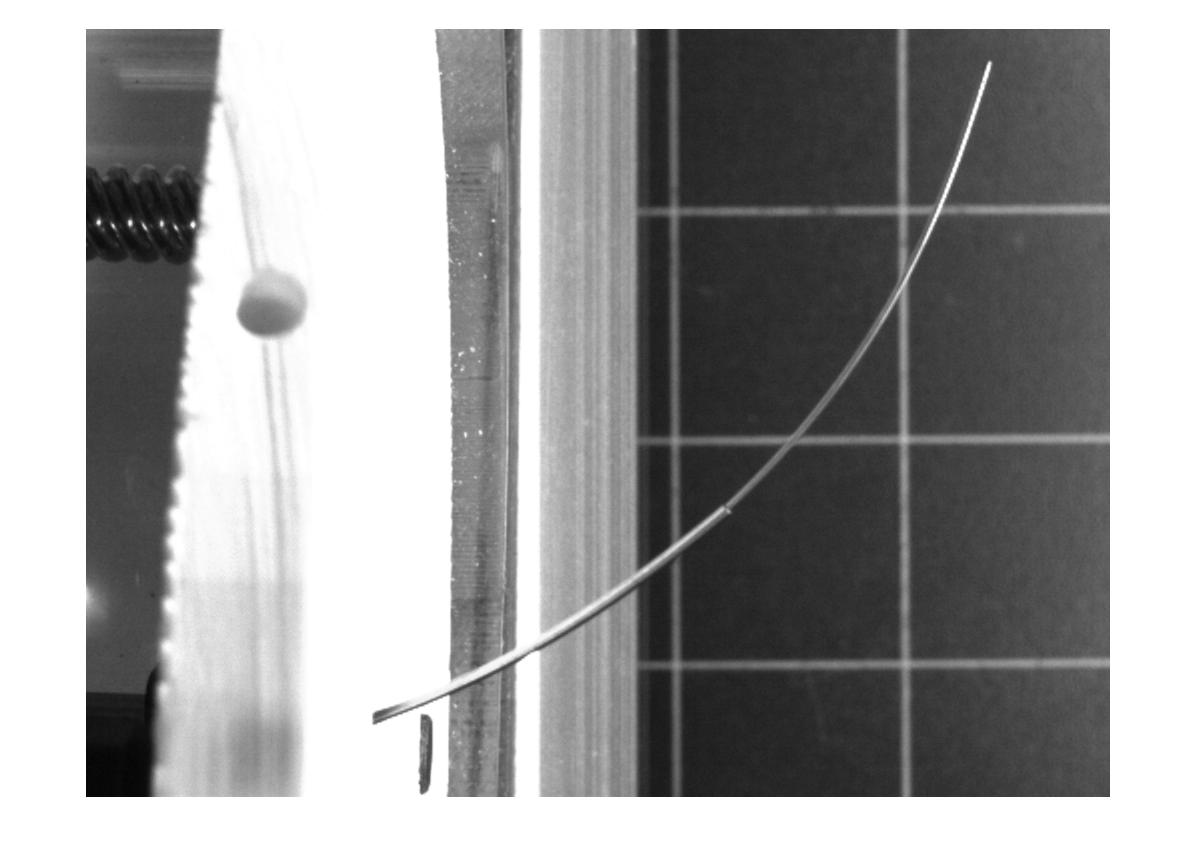
\includegraphics[width=\textwidth]{TP_1/curve1i.jpg}
         \caption{First image Tube}
         \label{fig:process1}
     \end{subfigure}
     \hfill
     \begin{subfigure}[b]{0.3\textwidth}
         \centering
         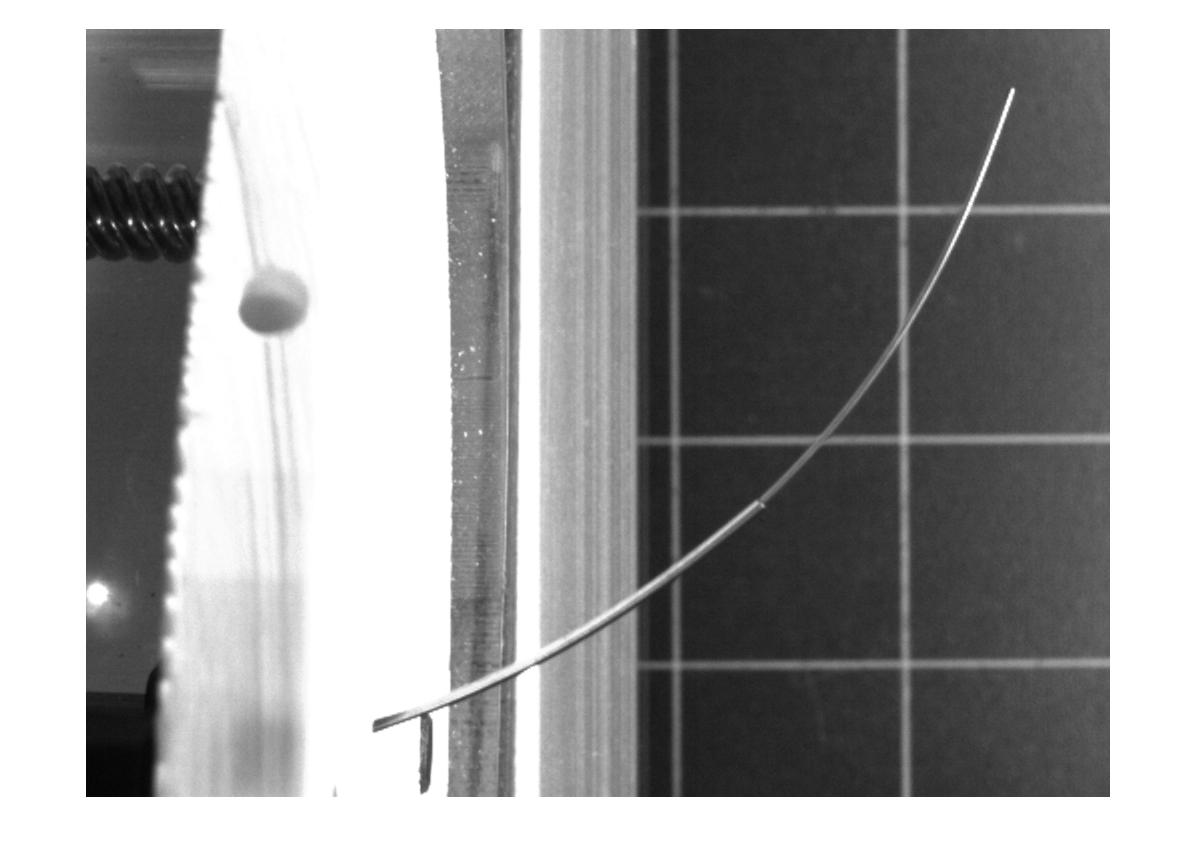
\includegraphics[width=\textwidth]{TP_1/curve2i.jpg}
         \caption{Second image Tube}
         \label{fig:process2}
     \end{subfigure}
     \hfill
     \begin{subfigure}[b]{0.3\textwidth}
         \centering
         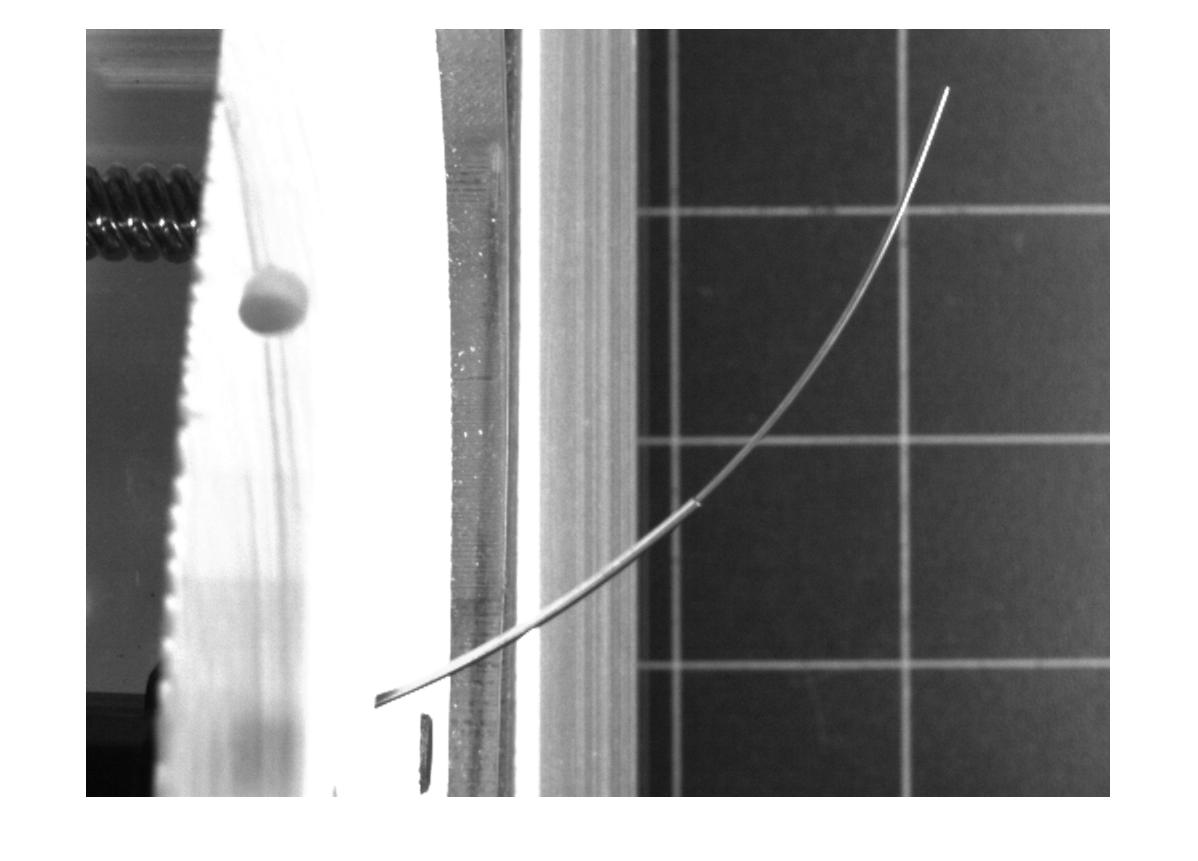
\includegraphics[width=\textwidth]{TP_1/curve3i.jpg}
         \caption{Third image Tube}
         \label{fig:process3}
     \end{subfigure}
      \hfill
     \begin{subfigure}[b]{0.3\textwidth}
         \centering
         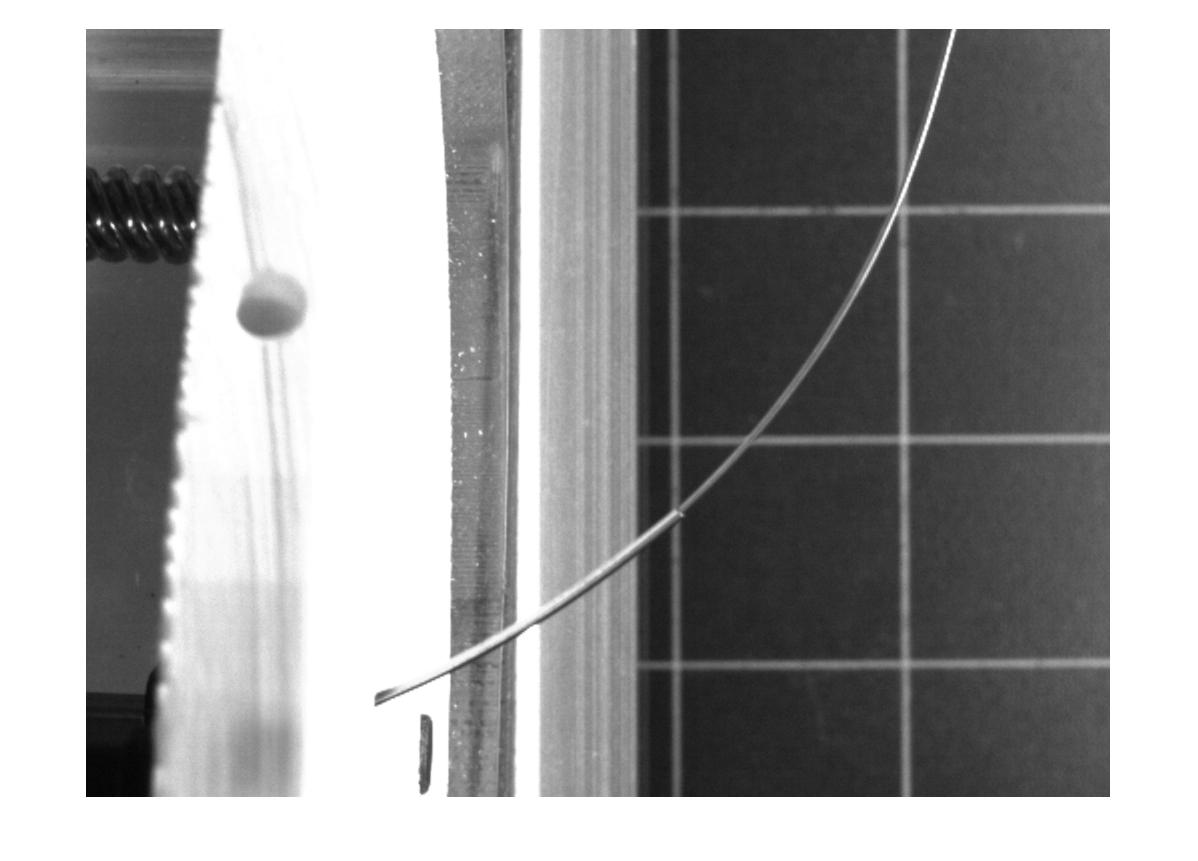
\includegraphics[width=\textwidth]{TP_1/curve4i.jpg}
         \caption{forth image Tube}
         \label{fig:process4}
     \end{subfigure}
      \hfill
     \begin{subfigure}[b]{0.3\textwidth}
         \centering
         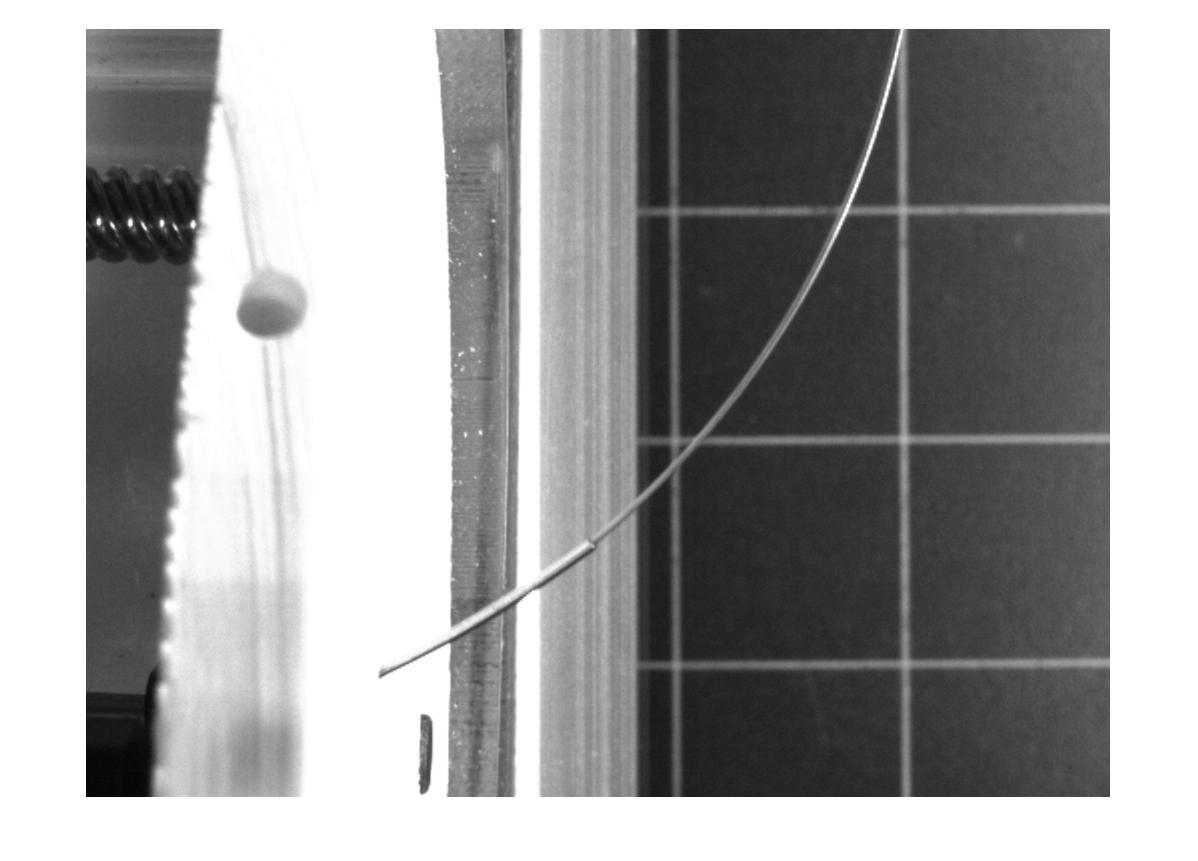
\includegraphics[width=\textwidth]{TP_1/curve5i.jpg}
         \caption{fifth image Tube}
         \label{fig:process5}
     \end{subfigure}
        \caption{Images processed}
        \label{fig:process}
\end{figure}
In Fig. \ref{fig:process}, the samples of the tubes are observed for the calculation of the curvature using the $ginput$ function, so using this function we can make a prediction of the possible curvature for each image, it is possible in each image to observe the different sections of each tube in the same way.



\begin{figure}[H]
     \centering
     \begin{subfigure}[b]{0.5\textwidth}
         \centering
         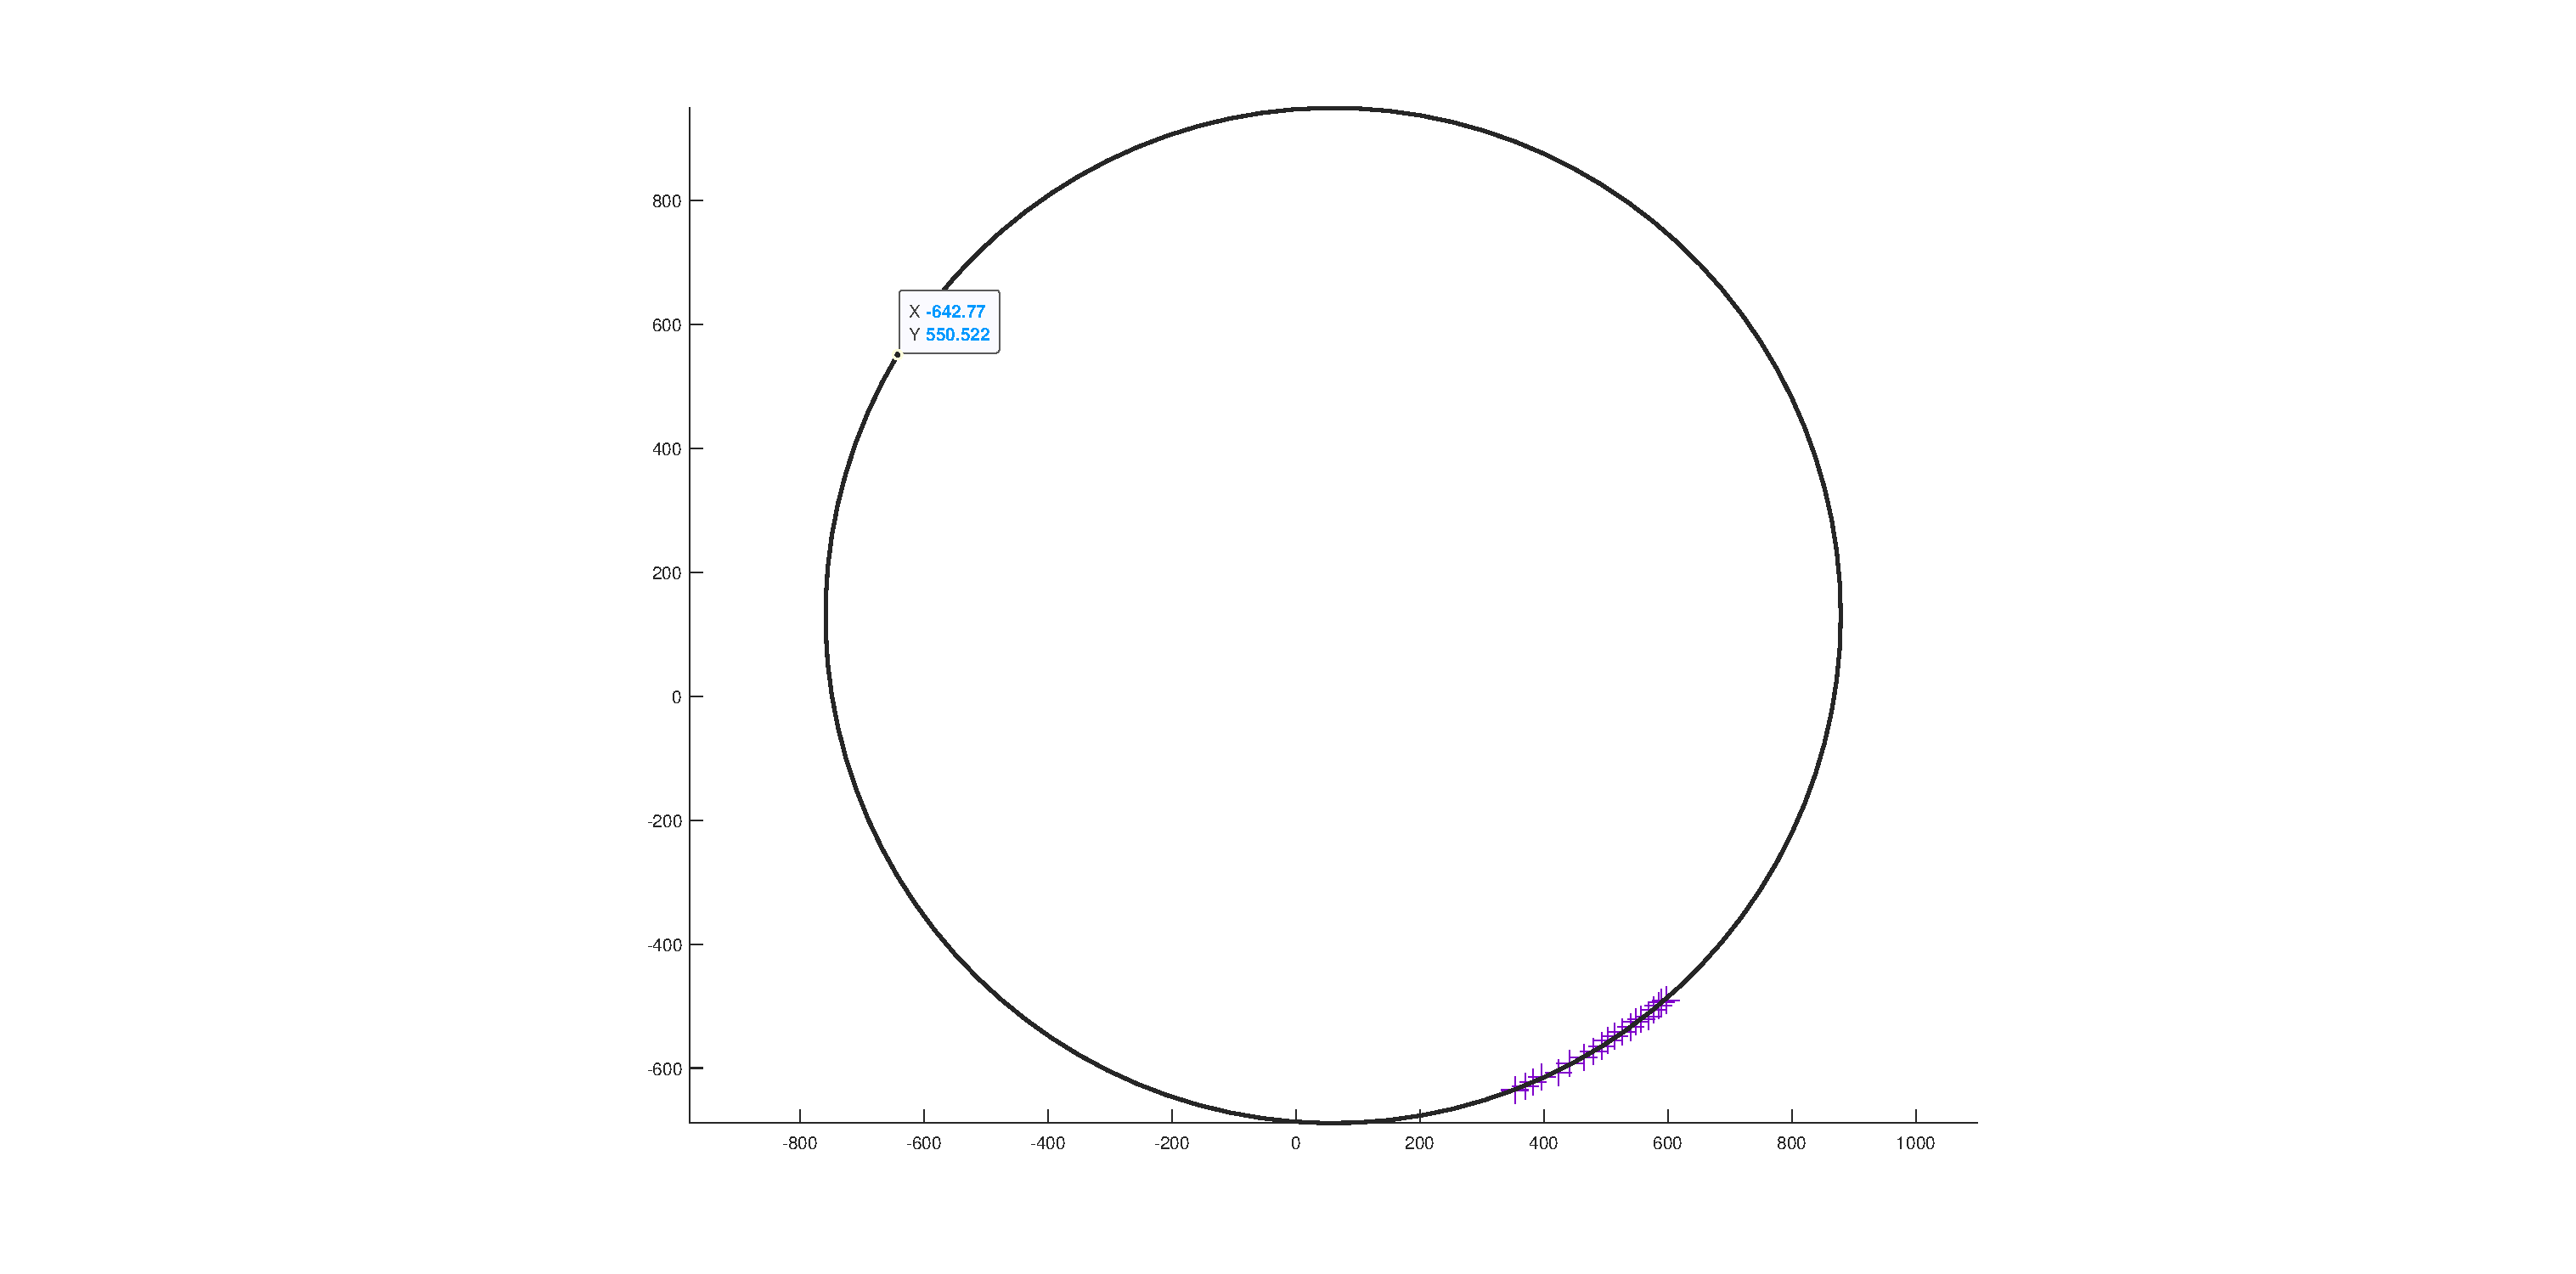
\includegraphics[width=\textwidth]{TP_1/curve1.eps}
         \caption{First Tube}
         \label{figtube1}
     \end{subfigure}
     \hfill
     \begin{subfigure}[b]{0.5\textwidth}
         \centering
         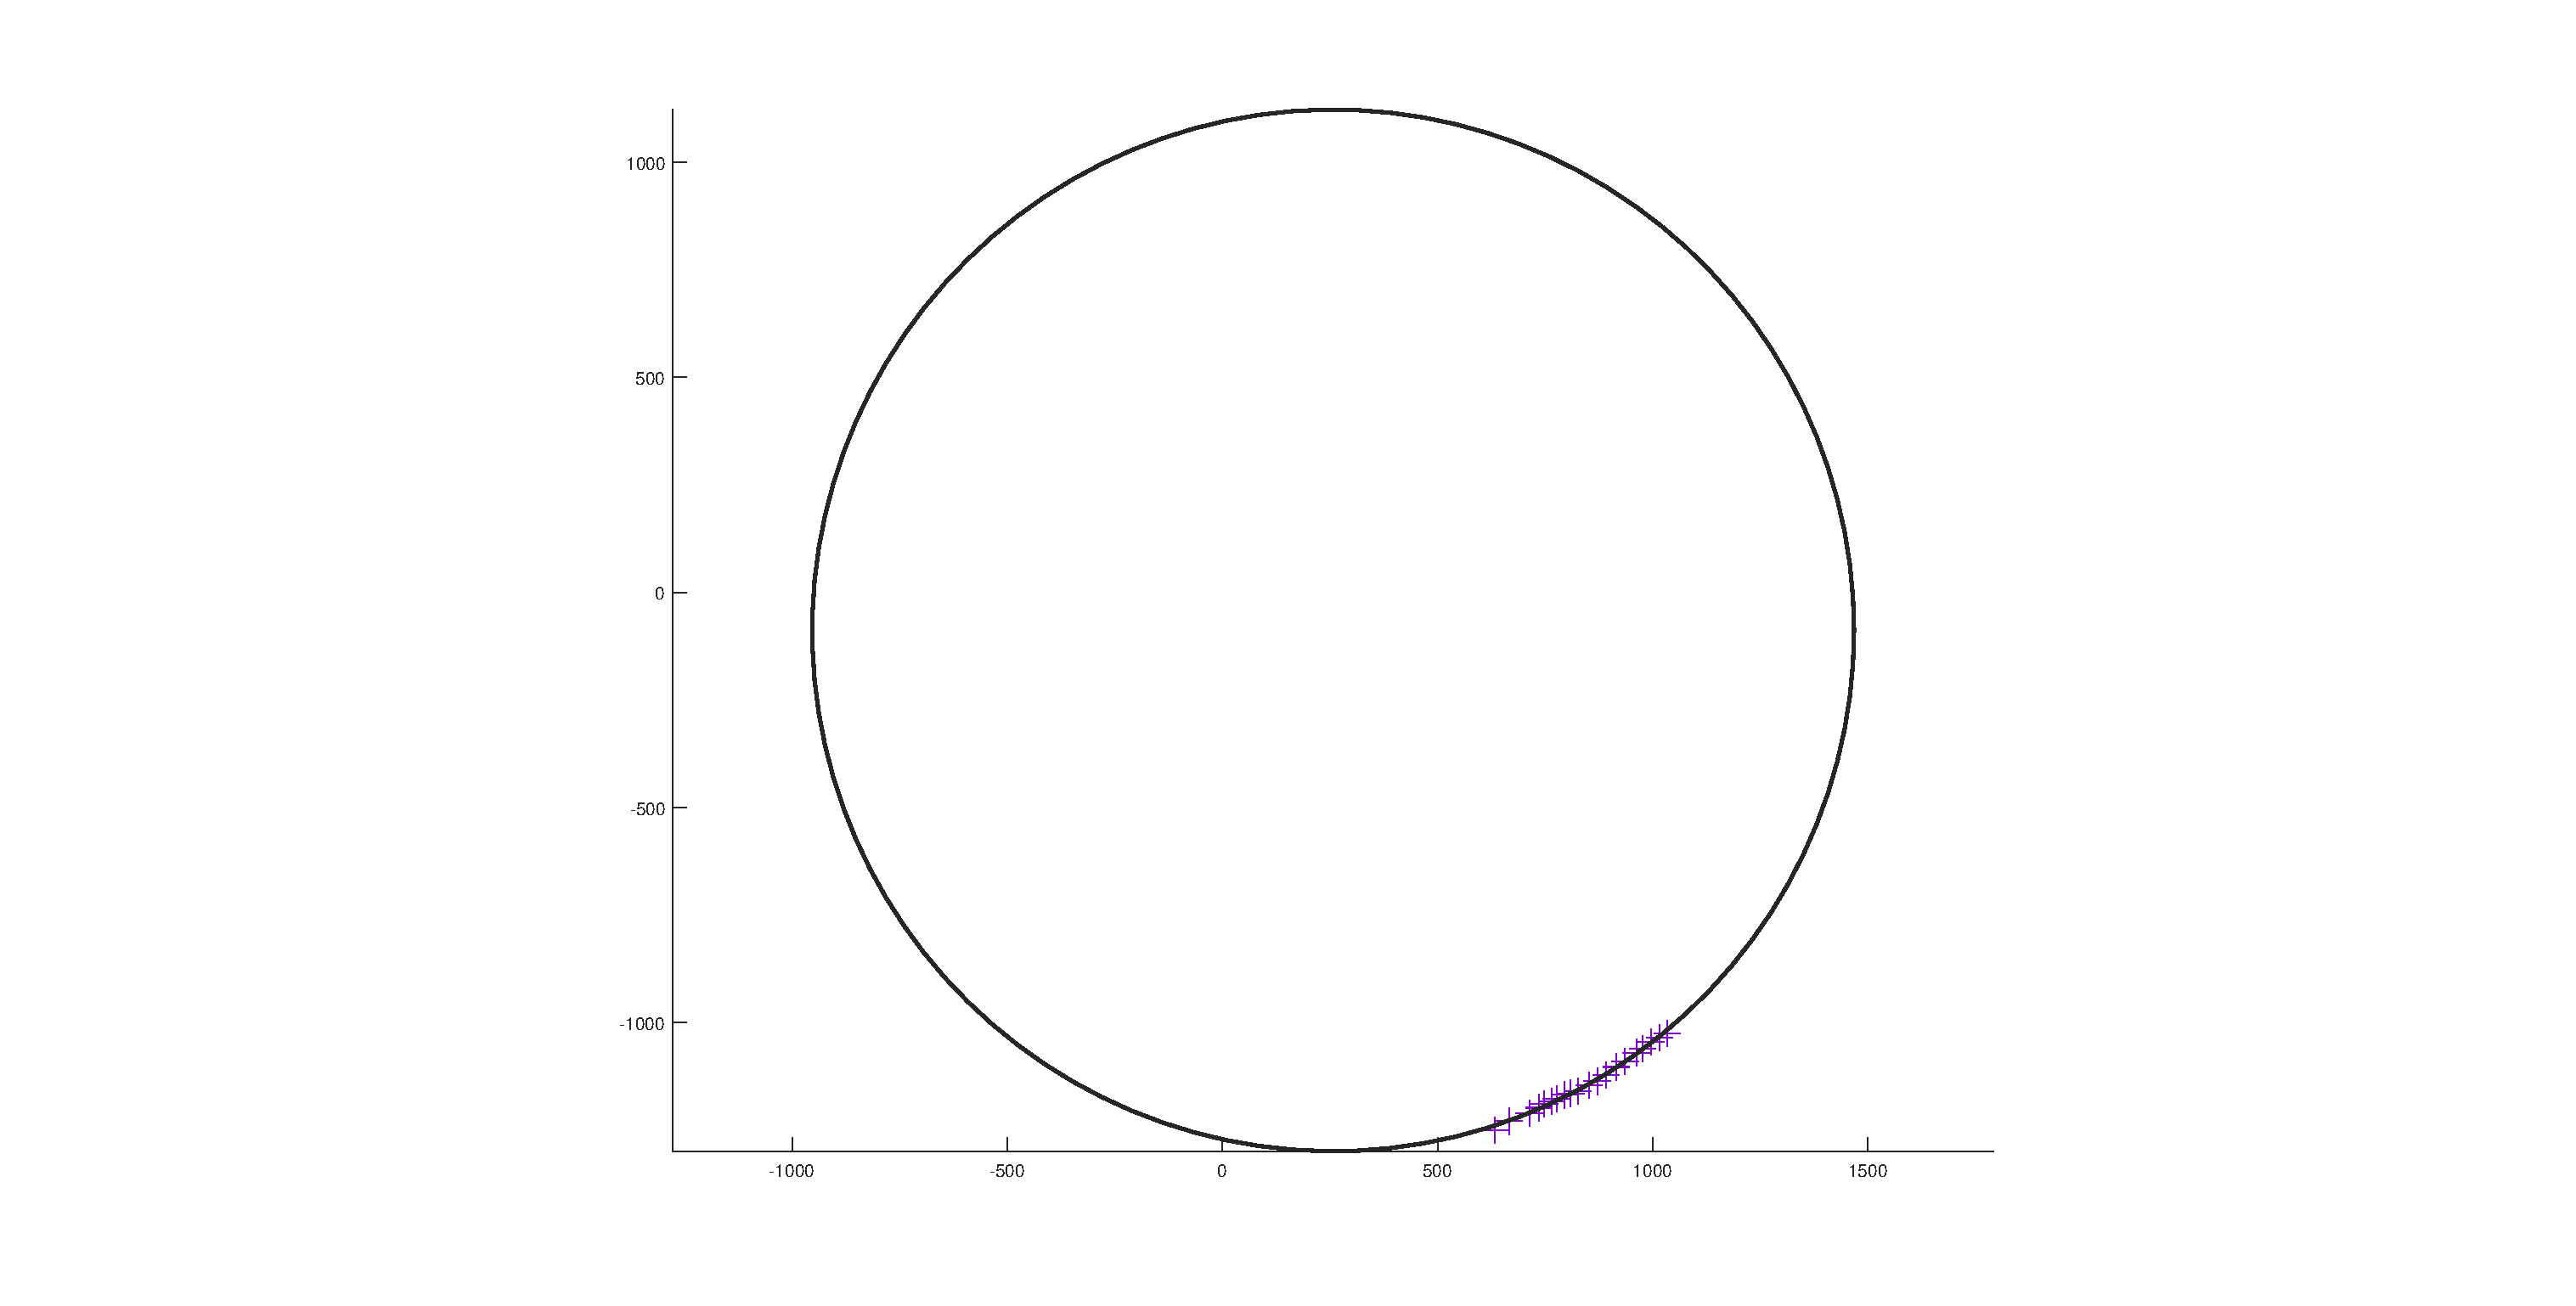
\includegraphics[width=\textwidth]{TP_1/curve2.eps}
         \caption{Second Tube measurement result}
         \label{fig:tube2}
     \end{subfigure}
     \hfill
     \begin{subfigure}[b]{0.4\textwidth}
         \centering
         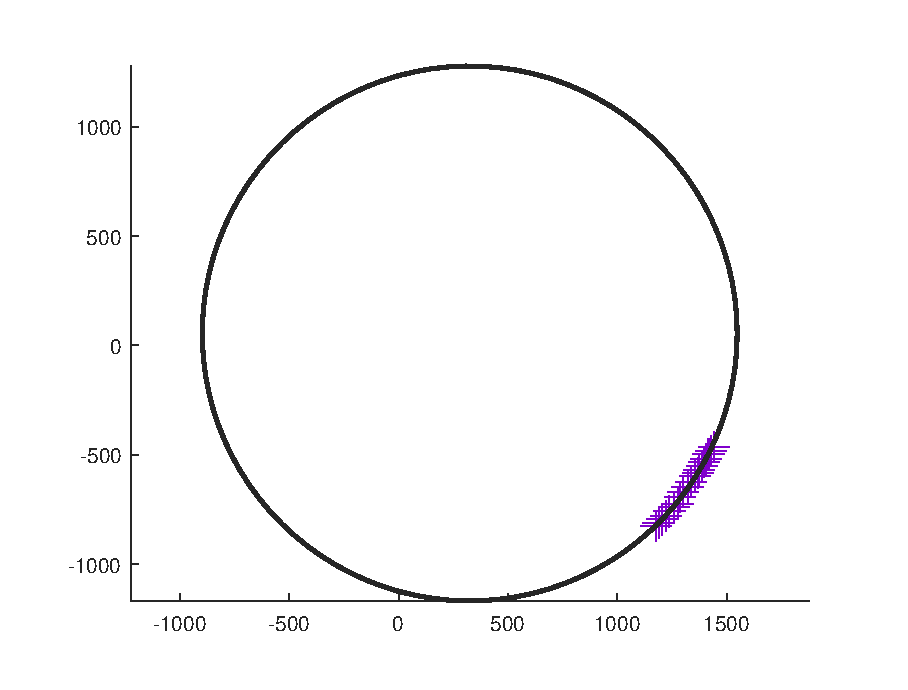
\includegraphics[width=\textwidth]{TP_1/curve3.eps}
         \caption{Third Tube measurement result}
         \label{fig:Tube3}
     \end{subfigure}
      \hfill
     \begin{subfigure}[b]{0.4\textwidth}
         \centering
         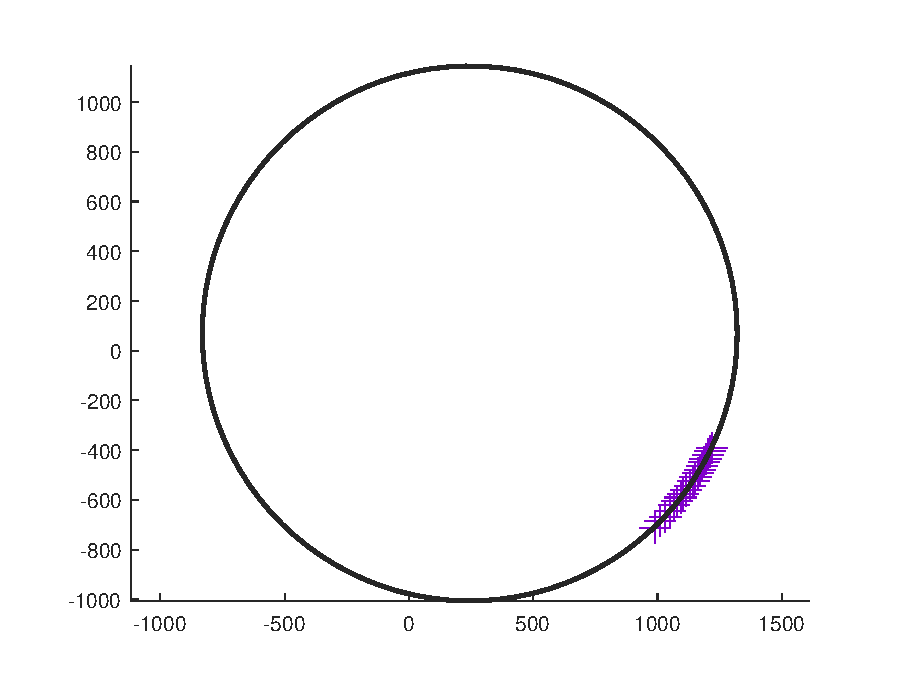
\includegraphics[width=\textwidth]{TP_1/curve4.eps}
         \caption{forth Tube measurement result}
         \label{fig:Tube4}
     \end{subfigure}
      \hfill
     \begin{subfigure}[b]{0.4\textwidth}
         \centering
         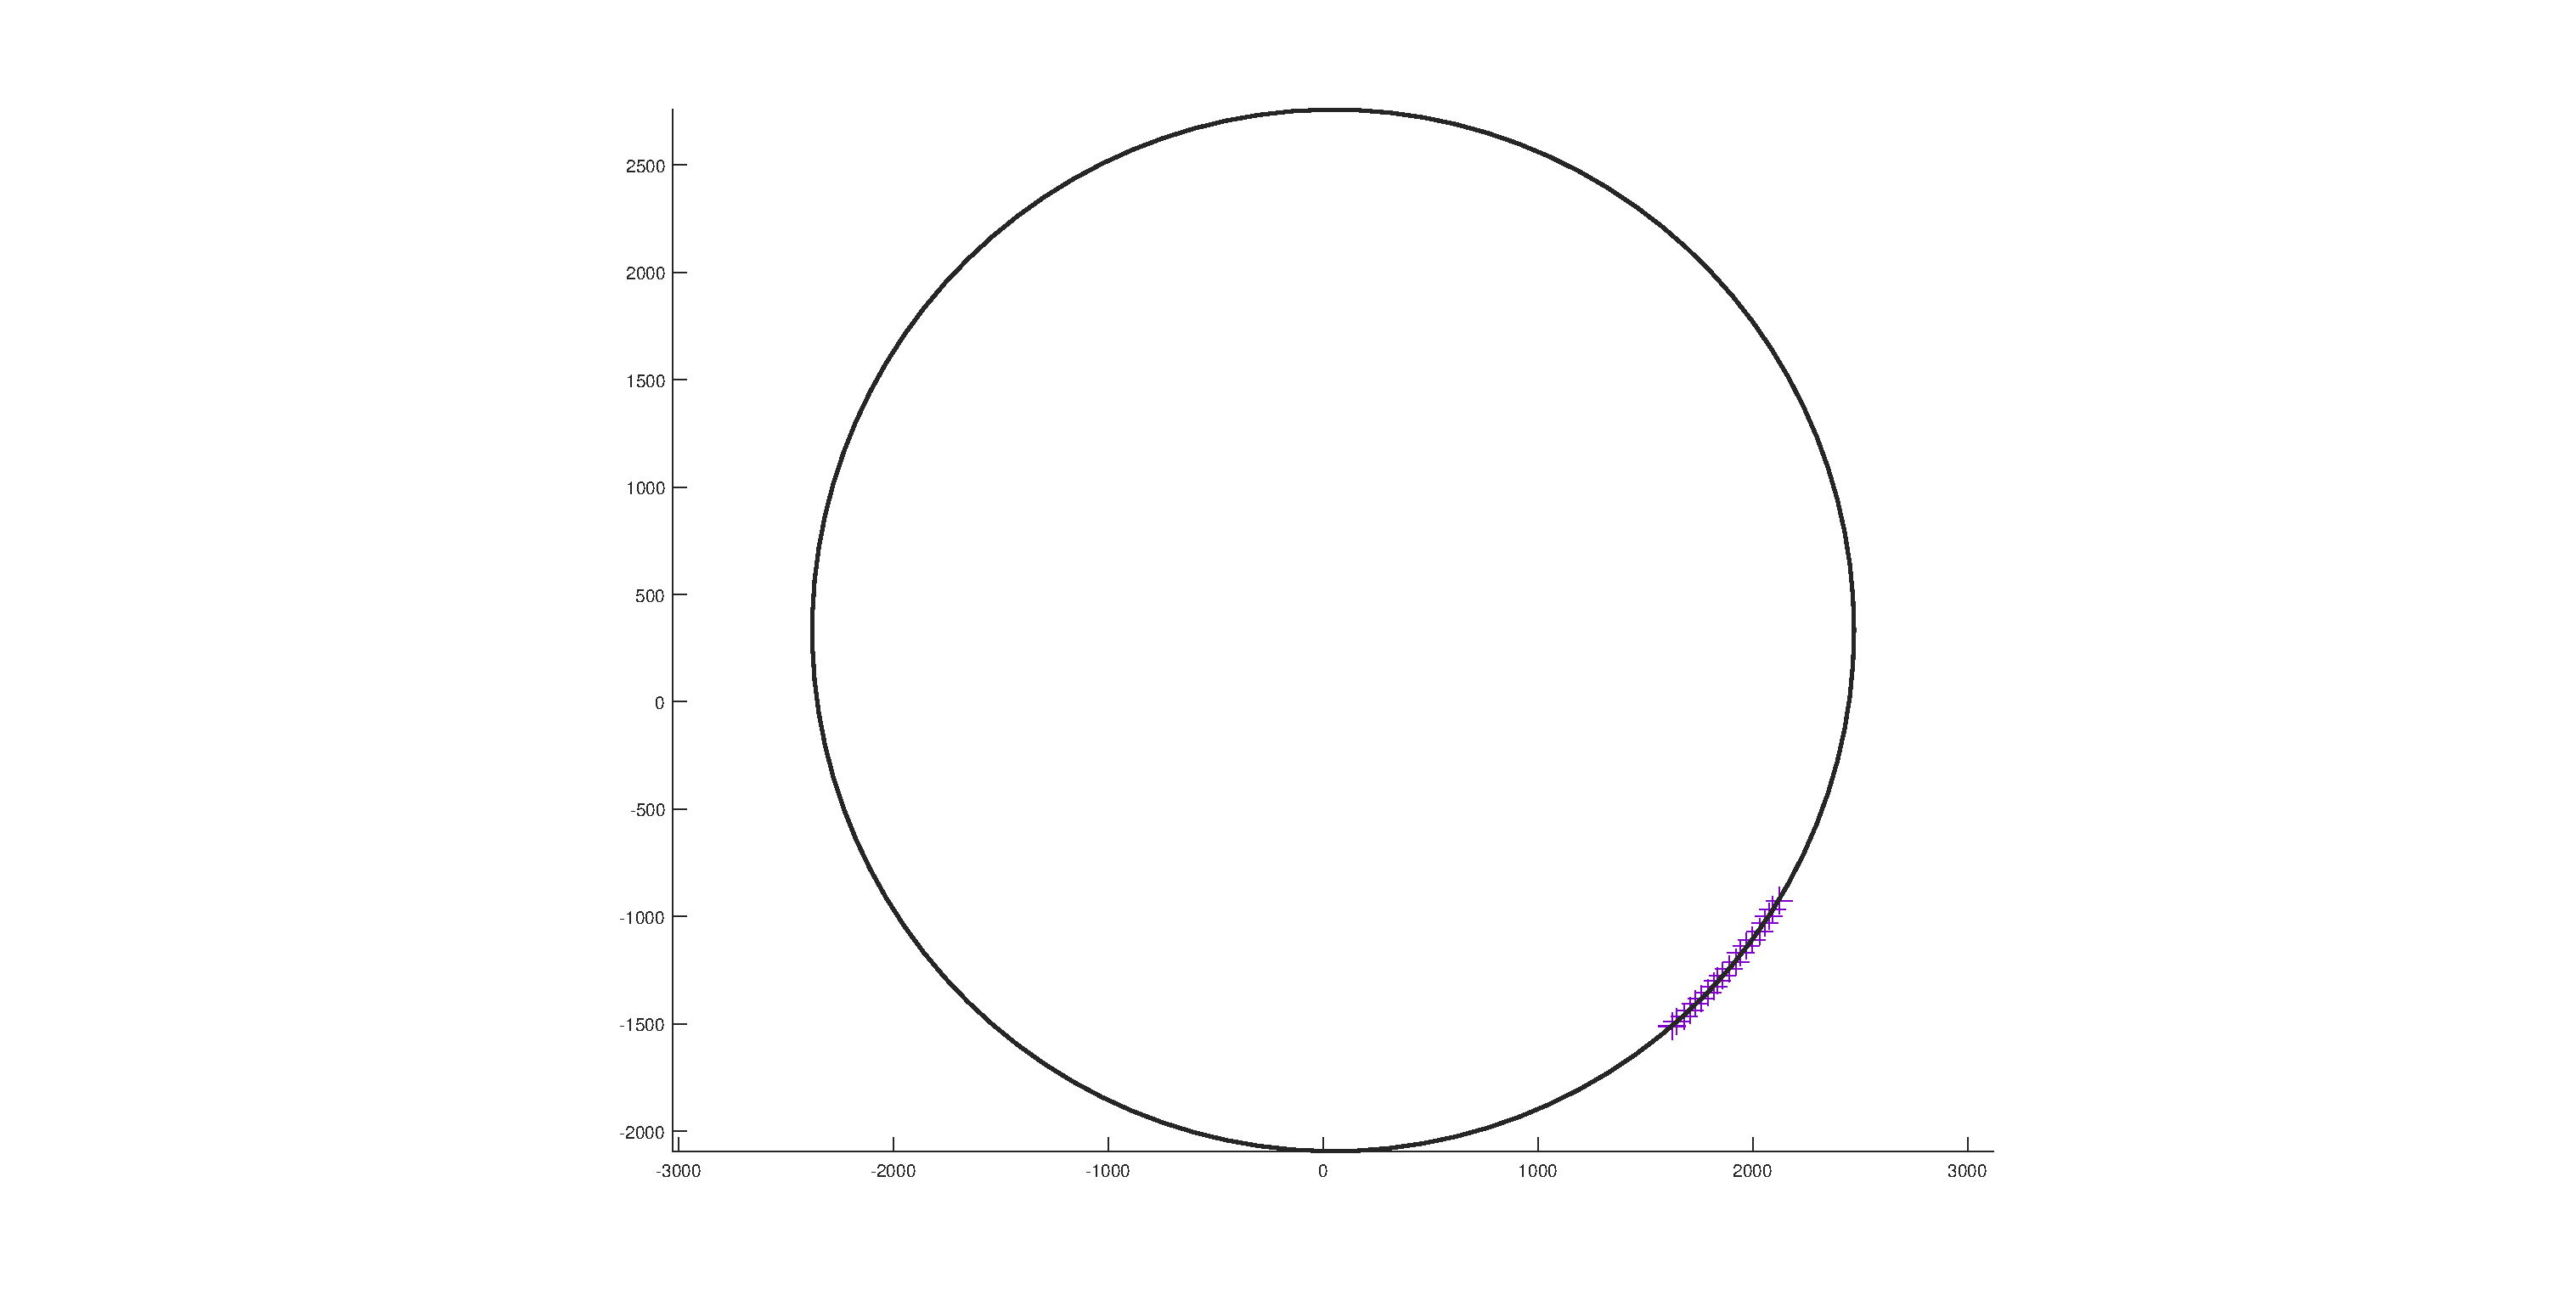
\includegraphics[width=\textwidth]{TP_1/curve5.eps}
         \caption{fifth Tube measurement result}
         \label{fig:Tube5}
     \end{subfigure}
        \caption{5 tubes measurement}
        \label{fig:tubes}
\end{figure}
In the Fig. \ref{fig:tubes}, it is possible to observe the measurements of the different configurations of tubes, each configuration was measured from 20 points which were selected from the functions provided in the sessions.
\begin{table}[H]
\caption{Table of Data}
\begin{tabular}{|c|c|c|c|}
\hline 
{\ul \textbf{Configuration}} & {\ul \textbf{mm to px ref. Point}} & {\ul \textbf{Curvature Radius}} & {\ul \textbf{Curvature}} \\ \hline
\textbf{1}                   & {[}29.4 -5.88{]}                   & $1x0558x10^3$                   & 0.9471                   \\ \hline
\textbf{2}                   & {[}28.46 -9.48{]}                  & $4.25x10^3$                     & 0.2351                   \\ \hline
\textbf{3}                   &  {[}22.77 -19.52{]}                              &     $1.28x10^3$                            &                 0.7772    \\ \hline
\textbf{4}                   & {[}29.69 -4.24{]}                                   &      $1.6983x10^3$                     &          0.5888           \\ \hline
\textbf{5}                   & {[}24 -18{]}                 &   $4.3348x10^3$           & 0.2307                         \\ \hline
\end{tabular}
\end{table}

Finally, in the previous table, we can observe the results of the curvature calculation for the tube, so it is possible to see how the first tube has the most significant curvature, which is shown according to the previously processed images.
\section{Exercise 3. Stability issue}
unfortunately, since the platform was down hence experimental evidence was not possible to obtain, we can only rely on the literature to discuss the stability of such systems.
With respect to the instability issues, we can observe the instabilities occurs when for example the two tubes are linked together, and any movement of one tube affects the other. This makes the robot inherently unstable and difficult to control. An instability occurs when this energy is rapidly released, and the robot “snaps” to a new configuration. Unforeseen snapping is clearly not desirable and could be dangerous in surgical applications.\\ 
on the other hand, we can also observe singularities based on the stiffness matrix of the architecture, where its possible to observe when the robot losses Degrees of Freedom and losses mobility. In the said matrix, we also see the presence of a lot of trigonometric functions (sin and cos) that are also causes of non-linearity and thus might induce instability.

\section{Conclusion}
In conclusion, the practical work on a concentric tube robot highlights the design and implementation of a robotic system that utilizes concentric tubes for its movement. We were able to calculate the transformation matrix for such type of robot and hence its kinematic model that differs from other robots, as a concentric tube can be considered as a serial robot with an infinite number of joints. We could see that by using just a image sample of the section we can reverse engineer the data and can deduce the configuration after calculating the configuration.\\
Unfortunately since we could not perform practical text, we only relied on literature and deduction to discuss the instability of such systems. it is worth mentioning that a somehow instability and some singularities on concentric tube models do not effect as much  it's accuracy as it is still one of the most accurate type of robots.

\chapter{TP 2: \LARGE Modeling and Calibration of a Parallel Micromanipulator }
A parallel robot is a mechanical structure, bases in different close chains kinematics, there is existing different type of architectures, defined principally in the type of architecture such as the $Spherical Parallel Robots$, \textit{Hybrid parallel robots} and the conventional architectures such as the Stewart Platform, which is the fundamental architecture for the hexapod presented in this work.\\
Finally the \textit{BORA} hexapod, its a platform controlled by a panel and a supervisory PC, the company provides for this robots a limited information data, where is possible to find the technical data as the torques and the size of the robot.

\section{First Approach of The Device}

\subsection{\textbf{Question 1:} Analyze the Mechatronic architecture of the system, specifying the role of each
element. A diagram might be useful}

The hexapod presented in the practical session in the field of parallel robots is called \texttt{6-U \barbelow{P} S}, which means 6 actuators$i=6$, an universal joint with 2$DoF$ for each one, a prismatic actuator, and a spherical joint with 3$DoF$. 


\begin{figure}[H]
     \centering
     \begin{subfigure}[b]{0.5\textwidth}
         \centering
         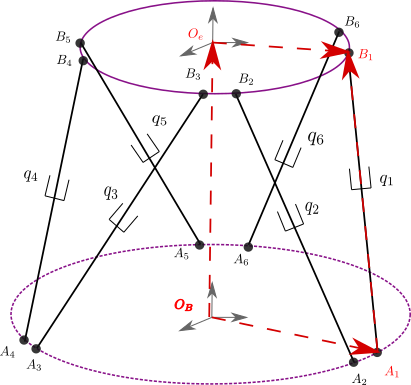
\includegraphics[width=\textwidth]{TP_2/diagram1_stewart.png}
         \caption{Diagram Representation}
         \label{fig:st1}
     \end{subfigure}
     \hfill
     \begin{subfigure}[b]{0.5\textwidth}
         \centering
         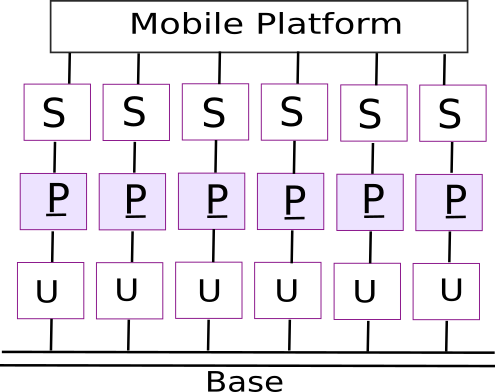
\includegraphics[width=\textwidth]{TP_2/stewartjoints.png}
         \caption{Joint Configuration}
         \label{fig:st2}
     \end{subfigure}
        \caption{Architecture of Stewart Platform}
        \label{fig:stt}
\end{figure}
The schema for this parallel robot is observed in the Fig. \ref{f   ig:st1}, where we have defined the Universal passive joints as $A_i$, the spherical passive joints as $B_i$, the prismatic active joints $q_i$ and finally Base reference $O_B$ Frame and a mobile reference $O_e$ for the Mobil platform. \\
In order to specify the role of each element, we can define the kinematic chain of the robot presented in the Fig. \ref{fig:st2}, where we can the connection between the mobile and the base platform, the universal joint $A_i$ is connecting the base platform, the Spherical joint $B_i$ connects the Mobil platform, the Active joint $P$ is the actuated joint and the mobile platform $O_p$ is the manipulated platform.


\subsection{\textbf{Question 2:} Find in the documentation the technical data (strokes, dimensions, resolution,
repetitiveness, etc.) of the robot. In particular, experimentally verify the dimensions of the
workspace.}

In order to analyze the technical data of the Hexapod, we can find the datasheet in \footnote{Technical date of the Hexapod: \url{https://symetrie.fr/hexapodes/bora/}.}, where its possible to observe the key features of this platform. 
\begin{figure}[H]
    \centering
    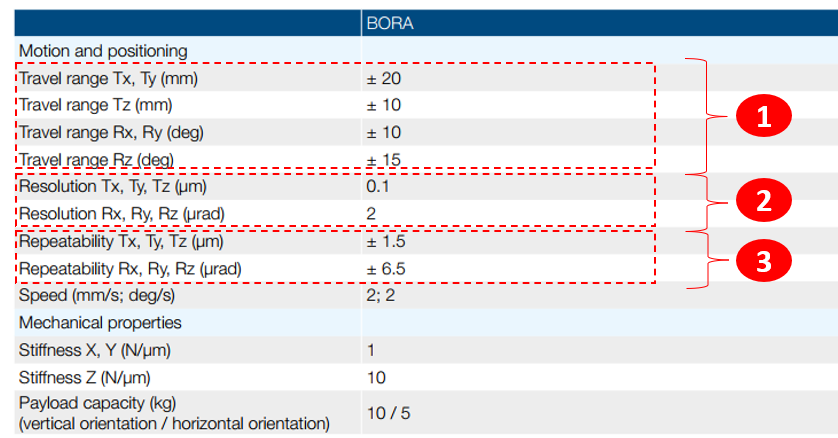
\includegraphics[width=\textwidth]{TP_2/charact1.png}
    \caption{ Technical Data of the Hexapod}
    \label{fig:char1}
\end{figure}
So that in the Fig. \ref{fig:char1}, its possible to observe the principal characteristics for this type of robot, firstly the travel range  in \textbf{1} give us an approximation to the workspace, secondly in \textbf{2} the resolution of the platform shows the precision of the system, its interesting observe how the precision is defined as $\mu$ units, which shows a high precision compared with conventional serial robots, in the same way the repeatability in \textbf{3}, presents a good accuracy for this mechanism. 

\begin{figure}[H]
    \centering
    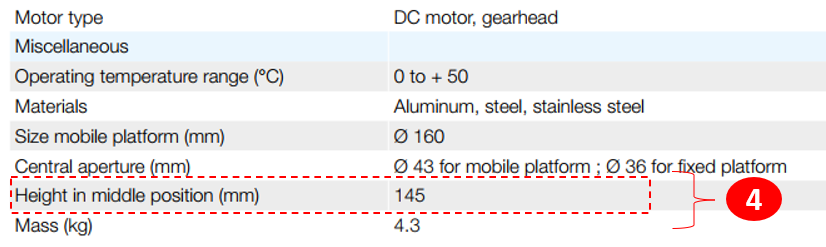
\includegraphics[width=\textwidth]{TP_2/charact2.png}
    \caption{Complementary Technical Data of the Hexapod}
    \label{fig:char2}
\end{figure}
Finally a geometric approximation is  presented in the data of Fig. \ref{fig:char2}, where its possible observe in \textbf{4} the height of the platform. 

\begin{figure}[H]
    \centering
    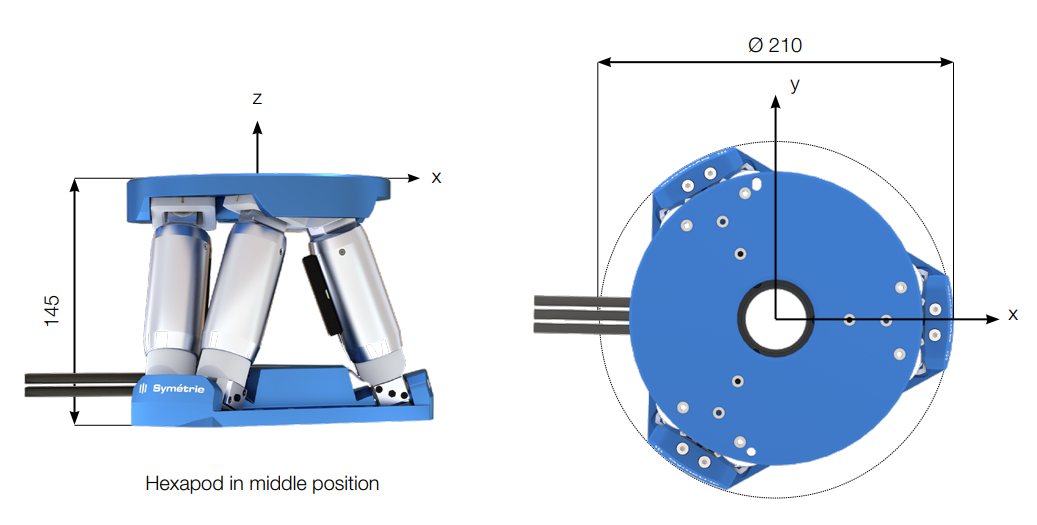
\includegraphics[width=\textwidth]{TP_2/hexapod1ac.png}
    \caption{Architecture of the hexapod}
    \label{fig:hexc1}
\end{figure}
Therefore in Fig. \ref{fig:hexc1}, we can observe the reference dimension of the Hexapod, where we can see how the maximum height of the platform with a value of 145 give us a reference of the size of this platform.
    


\subsection{Question 3: Can we easily ensure resolution and repeatability? Make a montage allowing the best possible measure.}

Yes, we can easily ensure the resolution and repeatability, by making a montage, we can create a more accurate measurement. Furthermore, by using sensor-based control and camera calibration for visual control in conjunction with the hexapod robot, this is how parallel robots in many cases can be used for \textit{micro-manipulation tasks}.

\section{Calibration Method}

\section{Writing of the classical model}
\subsection{Question 4}
\textbf{Considering the leg i of the mechanism, show that the implicit geometric model as a
function of the articular variable $q_i$, of the pose of the effector in the base reference mark $^b T_e$ and
coordinates of the points of attachment of the leg on the base $^b A_i$ and on the mobile platform $^e B_i$ is
written:}\\


In order to reduce to the implicit geometric model, we need to use the close loop chain of the Haxapod defined in:\\
\begin{figure}[H]
    \centering
    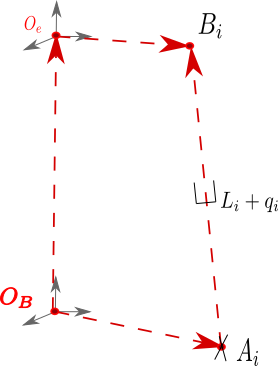
\includegraphics[height=7cm, width=4cm]{TP_2/close_loop.png}
    \caption{Close Loop chain}
    \label{fig:close_loop}
\end{figure}
Therefore there is possible to use vector operations, which will provide us:\\
\begin{center}
    $^b \Vec{OE} = ^b \Vec{OA_{i}} + ^b\Vec{A_i B_i} + ^b \Vec{B_i E} $\\
    $\Vec{A_i B_i} = (L_i + q_i)\Vec{u}$\\
    $( ^b \Vec{A_i} - ^b T_{e}* ^e B_{i} )^2 = (L_{i}+ q_{i}) \Vec{u} $\\
    $(q_{i} + L_{i})^2 = ||^b \Vec{A_i} - ^b T_e * ^e B_i||$
    
\end{center}


\begin{equation}
     (q_i+L_i)^2=||{}^b \~ A_{i} - {}^b T_{e} {}^e \~ B_{i}||^2
\end{equation}



\subsection{Question 5}
Reduce the inverse geometric model.\\
\begin{equation}
    q=g(X, \zeta)
\end{equation}

\begin{equation}
    \forall i =1..6, (q_i+L_i)^2=||{}^b \~ A_{i} - {}^b T_{e} {}^e \~ B_{i}||^2
\end{equation}
\begin{equation}
    q_{i}=||{}^b \~ A_{i} - {}^b T_{e} {}^e \~ B_{i}|| - L_i 
\end{equation}

\subsection{Question 6}
Suggest a method to solve the direct geometric problem.\\ 

\begin{itemize}
    \item Find the implicit kinematic model and solve the inverse
kinematic model of each leg in order to Extract the forward geometrical
model from the inverse kinematic model.

\item The method of the spheres.
\end{itemize}
\section{Writing the model in the measured Frame}
\subsection{Question 7}
Show that the implicit geometric model is written as a constraint, for each leg $i$,
between $q_i$, the pose provided by the exteroceptive sensor ${}^c T_m$ and the coordinates of the points $A_i$
and $B_i$ expressed in the appropriate landmarks.

\begin{equation}
    \forall i =1..6, (q_i+L_i)^2 - ||{}^b \~ A_{i} - {}^b T_{e} {}^e \~ B_{i}||^2=0
\end{equation}
In this way, we can transform using the equation:\\
\begin{equation}
    {}^b T_{e}=\begin{bmatrix}
{}^c R_{m} & {}^c t_{m} \\
0 & 1 
\end{bmatrix}
\end{equation}



\subsection{Question 8}
What are the parameters to be estimated during calibration?\\
The parameters to find are the static parameters as the offset of the prismatic joint, The distance between the joints and the Mobil platform, the distance between the base platform and the joints.
\subsection{Question 9}
Show that calibration can be done for each leg independently of the others. \\
The calibration can be done independently because the hexapod forms 6 independent close loops, that depends of:
\begin{itemize}
    \item Arm Value
    \item Normal Vector
    \item Constant in the robot frame
\end{itemize}

\begin{figure}[H]
     \centering
     \begin{subfigure}[b]{0.3\textwidth}
         \centering
         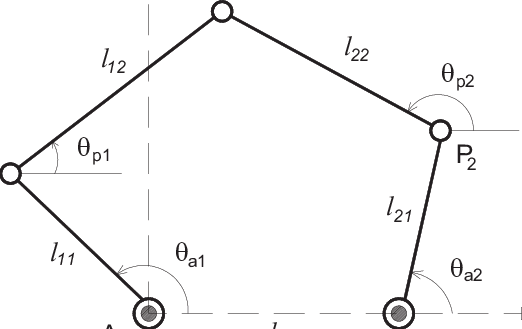
\includegraphics[width=\textwidth]{TP_2/parallel1.png}
         \caption{Planar parallel robot }
         \label{fig:st1a}
     \end{subfigure}
     \hfill
     \begin{subfigure}[b]{0.3\textwidth}
         \centering
         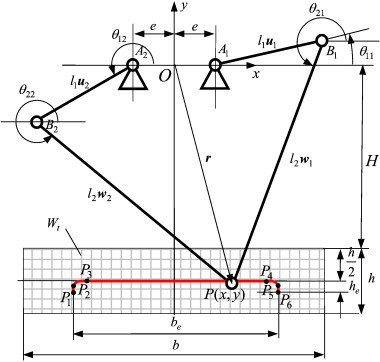
\includegraphics[width=\textwidth]{TP_2/parallel2.jpg}
         \caption{Delta Robot}
         \label{fig:st2a}
     \end{subfigure}
        \caption{parallel robots}
        \label{fig:stta}
\end{figure}
As is observable en the Figs. \ref{fig:st1a} and \ref{fig:st2a}, we have different architectures with close chain configurations, but for each case we can do independently the calibration Process.
\subsection{Question 10}
There is existing several methods for non linear optimization, some of the most popular are:\\

\begin{itemize}
    \item  Gradient descent
    \item Newton's Method
    \item  Conjugate gradient
\end{itemize}

In order to find to do optimization in this work we are using the \textit{Gradient descent} method.\\
The gradient descent algorithm is a nonlinear optimization algorithm that finds the minimum of a function by moving in the direction of the negative gradient of the function.\\
In this way the steps in order to use this method are:\\

\begin{itemize}
    \item Choose the appropriate function to minimize.
    \item Choose the starting point.
    \item Choose the number of iterations.
    \item Choose the tolerance.
    \item Perform the iterations.
\end{itemize}


\subsection{Question 11}


In order to derive the jacobian matrix, firstly we need recall the implicit form equation of the kinematic close chain in Eq. \ref{eq:implicit2}, where its possible to observe the parameters for each length, as the distance between the joints and the references and the Mobil joints expressed with $q_i$. 
\begin{equation}
    \forall i =1..6, f = (q_i+L_i)^2 - ||{}^b \~ A_{i} - {}^b T_{e} {}^e \~ B_{i}||^2
    \label{eq:implicit2}
\end{equation}
Secondly we are defining the variables to optimize, in this case according with the instructions we are optimizing the offset length $L_i$, the distance between the passive joints and the Mobil platform defined as $^c A_i$, the distance between the passive joints and the frame reference $^m B_i$.  So that, the Jacobian will be defined as:\\
\begin{equation}
    J=[\dfrac{df}{L_{i}} \quad \dfrac{df}{{}^c A_{i}} \quad \dfrac{df}{{}^m B_{i}}]
    \label{eq:jac}
\end{equation}

For each component we can define the partial differentiation as:\\
\begin{center}
    $\dfrac{df}{L_{i}}=2*(q_i + L_i)$\\
    $\dfrac{df}{{}^c A_{i}}= -2* ||^c A_{i} - ^c R_{m}* ^m B_{i} - ^c T_{m} || $\\
    $\dfrac{df}{{}^m B_{i}}=2* ^c R_m *(|| ^c A_{i} - ^c R_{m}* ^m B_{i} - ^c t_{m} ||)$
\end{center}

In consequence with the Eq. \ref{eq:jac}, additionally its possible to find the changes in the implict model.
\subsection{Question 16}
Write the function \textit{$MGI_indiv$} which calculates the deviation to the geometric model
implicit for ONE leg i, A configuration of the platform and an estimate current of the geometric
parameters of the leg considered.\\
\begin{lstlisting}
    function [ ecarti ] = MGI_indiv(qi, cTm, param_i) %% Function to calculate the cost function for each leg
    Li=param_i(1); %m %Length of the leg 
    cAi=param_i(2:4); %Parameter 1 to optimize 
    mBi=param_i(5:7); % Parameter 2 to optimize

    cRm=cTm(1:3,1:3);
    cTm1=cTm(1:3,4);
    %ecarti=(qi+Li)^2-norm(cAi-cRm*mBi -cTm1)^2; % ecarti is the cost funmction
    ecarti=(qi+Li)^2-norm(cAi-(cRm*mBi) -cTm1)^2; % ecarti is the cost funmction
end
\end{lstlisting}



Find Attached the implementation code, in the following link \footnote{Repository of the Tps \url{https://github.com/GroverAruquipa/Micro_robotics_TPs}.}

\subsection{Question 17}
Write the $Regresseur_indiv$ function which calculates the regressor for ONE leg and
ONE configuration of the platform.
\begin{lstlisting}
    function [ Jparam_i ] = Regresseur_indiv(qi, cTm, param_i) % function2
    Li=param_i(1); %m %Length of the leg 
    cAi=param_i(2:4); %Parameter 1 to optimize 
    mBi=param_i(5:7) ;% Parameter 2 to optimize
    cRm=cTm(1:3,1:3);
    cTm1=cTm(1:3,4);
    Li=40;
    J11=qi+Li;
    J22=-(cAi-cRm*mBi -cTm1)';
    J33=(cAi-cRm*mBi -cTm1)'*cRm;
    rest=(qi+Li)^2 - (norm(cAi -(cRm*mBi) - cTm1))^2;
    Jparam_i= rest*[J11 J22 J33];
    Jparam_i= [J11 J22 J33];
end
\end{lstlisting}

\subsection{Question 18}
 Write the total MGI function that calculates the vector of all deviations to the implicit
geometric model for ONE leg and ALL the configurations of the platform.
\begin{lstlisting}
    function [ Jparam_total ] = Regresseur_total(les_qi, les_cTm, param_i)
    for LegNo=1:40
        Jparam_i(LegNo,:)=Regresseur_indiv(les_qi(LegNo),les_cTm(:,:,LegNo),param_i);
    end
    Jparam_total=Jparam_i;
end
\end{lstlisting}

\subsection{Question 19}
Write the total regressor function which calculates the regressor of all the deviations
to the implicit geometric model for ONE leg and ALL platform configurations.
\begin{lstlisting}
    function [ Jparam_total ] = Regresseur_total(les_qi, les_cTm, param_i)
    for LegNo=1:40 Jparam_i(LegNo,:)=Regresseur_indiv(les_qi(LegNo),les_cTm(:,:,LegNo),param_i);
    end
    Jparam_total=Jparam_i;
end
\end{lstlisting}



\subsection{Question 20}
Write the nonlinear optimization calibration function.


For the non linear calibration function is used the descend of the gradient following the next steps:

\begin{equation}
    a_{i+1}=a_{i}- \alpha*\dfrac{dJ_{x1,xn}}{d_{x_n}}
    \label{eq:eq1des}
\end{equation}
So that, the algorithm for the descense of the gradient principally is based in an iteration where we need to reduce the error in the parameters calculated and measured, until to have a minimal error or a certain number of iterations, as is observed in the following peace of code.
\begin{lstlisting}
    function [ param_estimes_i conddtion_error counter] = etalonnage(les_qi, les_cTm, param_i_init)
% les qui is 40x6 
% les cTm is 4x4x40
% param_i_init is 6x1
% We neeed stimate the correct cAi and mBi for each leg
    Li=param_i_init(1); %m %Length of the leg 
    cAi=param_i_init(2:4); %Parameter 1 to optimize 
    mBi=param_i_init(5:7) ;% Parameter 2 to optimize
    alpha=0.1;
    % Regressor_indiv is the cost function to minimize
    % Regressor_indiv(les_qi,les_cTm,param_i)

    varaux=size(les_cTm);
    
    
    param_i=param_i_init';
    counter=1;
    conddtion_error=MGI_indiv(les_qi(1,1), les_cTm(:,:,1), param_i);
    %conddtion_error=50;
    while (1)
        counter=counter+1;
        Jcost=Regresseur_indiv(les_qi(1,1), les_cTm(:,:,1), param_i);
        %param_i
        %Jcost
        param_i_new=param_i - (alpha*Jcost)';
        % if param_i_new is NaN
        if isnan(param_i_new)
            param_i_new=param_i;
        end
        % if param_i_new is Inf
        if isinf(param_i_new)
            param_i_new=param_i;
        end 

        param_i=param_i_new
        conddtion_error=MGI_indiv(les_qi(1,1), les_cTm(:,:,1), param_i);
        conddtion_error
        %counter
        if counter>1000
            counter
            break
        end
        if conddtion_error<5 
            counter
            break
        end 
    end
    param_estimes_i=param_i;
   
end
\end{lstlisting}




\subsection{Question 21}
Apply the method to each leg for the sequence you recorded.\\
In the following script you can see the code developed for a leg, what you want to do here is firstly to search for the smallest of the samples taken, to then use the optimization function to calculate the next value, for this way to compare the error, using the cost function.

\begin{lstlisting}
   function [cond_error_vect param_estimes_i conddtion_error counter] = etalonnage2(les_qi, les_cTm, param_i_init)
    % les qui is 40x6 
    % les cTm is 4x4x40
    % param_i_init is 6x1
    % We neeed stimate the correct cAi and mBi for each leg
        Li=param_i_init(1); %m %Length of the leg 
        cAi=param_i_init(2:4); %Parameter 1 to optimize 
        mBi=param_i_init(5:7) ;% Parameter 2 to optimize
        alpha=0.1;
        % Regressor_indiv is the cost function to minimize
        % Regressor_indiv(les_qi,les_cTm,param_i)    
        varaux=size(les_cTm);    
        param_i=param_i_init';
        counter=20;
        conddtion_error=MGI_indiv(les_qi(1,1), les_cTm(:,:,1), param_i);
        %conddtion_error=50;
        close all
        cond_error_vect=[];
        while (1)
            counter=counter+1;
            %Jcost=Regresseur_indiv(les_qi(1,1), les_cTm(:,:,1), param_i);
            Jcost=Regresseur_total(les_qi, les_cTm, param_i); % 40x6 table
            conddition_error=MGI_total(les_qi, les_cTm, param_i); % 40x6 table
            %find the minor from conddition_error
            [minval, minind]=min(conddition_error); % minind is the index of the minor value
            minval=abs(minval); % we need the absolute value of the minor value
            % used mindind to find the correct Jcost
            Jcost=Jcost(minind,:); %
            % evaluate with the minor value of Jcost
            param_i_new=param_i-alpha*Jcost'; %
            conddition_error_new=MGI_total(les_qi, les_cTm, param_i_new);
            %conddition_error_new=abs(conddition_error_new);
            % if conddition_error_new is minor than conddtion_error
            % we update the param_i
            if min(conddition_error_new)<minval
                param_i=param_i_new;
                cond_error_vect=[cond_error_vect conddition_error_new];
            else
                alpha=random('unif',0.1,0.5);
            end
            if minval<5
                param_i_new;
                break
            end
            %counter
            if counter>1000
                counter;
                break
            end
        end
        conddtion_error=minval;
        param_estimes_i=param_i;
    end 
\end{lstlisting}


\subsection{Question 22}
Verify the relevance of the estimated parameters.\\
\textit{This section could not be carried out due to the lack of theoretical technical data for comparison and in the same way due to technical drawbacks that do not help the use of the hexapod.}

\begin{table}[H]
\begin{tabular}{|c|c|c|c|}
\hline
\textbf{}  & \textbf{L1} & \textbf{L2} & \textbf{L3} \\ \hline
\textbf{A}&     1.6,0.43,-3.48       & 1.6, 0.43,-3.48]            &  1.6,0.43,-3.48             \\ \hline
\textbf{B}& -1.6104, -0.4355, 3.46            &     -1.6301,-0.4855,4.16        & 2.0102,0.2355,3.46]                \\ \hline
\textbf{l} &      0.085       &    0.078         &     0.079             \\ \hline
\end{tabular}
\end{table}

\begin{table}[H]
\begin{tabular}{|c|c|c|c|}
\hline
\textbf{}  & \textbf{L4} & \textbf{L5} & \textbf{L6} \\ \hline
\textbf{A} &       1.43,0.46,-3.48      &   1.62,0.32,4.48,         &       1.8,0.52,2.9               \\ \hline
\textbf{B} & 2.0102,0.2355,3.46]            &  [1.3104,0.2355,3.36]           &      ----           \\ \hline
\textbf{l} &  0.082           & 0.081            &                         \\ \hline
\end{tabular}
\end{table}


The parameters estimated in the table above reflect the convergence through gradient descent, although the values $l_i$ show a correct approximation, since the coordinates of the vectors $B$ and $A$ are these vectors, they reach have a difficult way to validate, in such a way to see if it is possible to modify the algorithm. It was only validated with the error metric that when the error is less than 0.3 the algorithm for the iteration and to change the learning rate for the non-linear part.

\subsection{Conclusion}
In this practical work we explore the calibration of a parallel robot, where we were able to observe the analysis of the implicit geometric equations of this model, in the same way a calibration method through parameter estimation using inverse kinematics, in the results found it was observed that Coordinates were found that must be moved at distances with respect to the references of the mobile platform and base, so these results cannot be fully validated due to the fact that they do not have the theoretical results for comparison, despite having a convergence to zero. It is expected in the future to master this method, since it comes to present an intrinsic complication :)

    


\end{document}